\documentclass[11pt]{book}
\usepackage[utf8]{inputenc}	% Para caracteres en español

\usepackage[left=2.75cm,right=2.75cm,top=2cm,bottom=3cm]{geometry}
\usepackage{style}
\thispagestyle{fancy}
\title{Analyse II}
\author{Arthur Herbette \\
Prof. Lachowska Anna}

\begin{document}
\setcounter{section}{8}
\maketitle

\thispagestyle{empty}
\tableofcontents
\thispagestyle{empty}
\listoflectures

\chapter{Introduction}
Le but de se document est d'y faire un résumé qui se trouve entre les notes de Joachim Favre (Dont j'ai utilisé le template) et Les résumé des théorèmes disponible sur moodle. Je vais essayer de me tenir a environ une à $2$ pages par cours


\chapter{Equations différentielles ordinaires}
\lecture{1}{2025-02-17}{Equa Diff}{}
\section{Introduction aux équation différentielles} 
\begin{definition}
    \important{Une équation différentielle ordinaire} est une expression \[E(x, y, y', \dots, y^{(n)}) = 0 \]
    où $E$ est une expression fonctionnelle, $n \in \mathbb{N}_0$, et $y = y (x)$ est une fonction inconnue de $x$ .\\
    On cherche un intervalle ouvert $I \subset \mathbb{R}$ et une fonction $y : I \to \mathbb{R}$ de classe $C^n$ telle que l'équation donnée est satisfaite $\forall x \in I$.
\end{definition}
\begin{parag}{Equation à variable séparées} 
 Une équation à variables séparées est une équation du type $f(y)\cdot y' = g(x)$ est une \important{EDVS} où : 
 \begin{itemize}
     \item $f: I \to \mathbb{R}$ est une fonction continue sur $I \subset \mathbb{R}$
     \item $g: J \to \mathbb{R}$ est une fonction continue sur $J \subset \mathbb{R}$
 \end{itemize}
 Une fonction $y: J' \subset J \to \mathbb{R}$ de classe $C'$ satisfaisant l'équation $f(y)\cdot y' = g(x)$ est une solution
 \begin{subparag}{Remarque personnelle}
     \begin{framedremark}
         Ce type d'équation se résoudre relativement ``rapidement'' car on peut transformer le $y'$ en $\frac{dy}{dx}$ et ``mettre le $dx$ de l'autre côté'' : 
         \[f(y)\cdot\frac{dy}{dx} = g(x) \implies \int f(y)dy = \int g(x) dx\] 
         Et il suffit donc t'intégrer les deux côtés et le tour est joué.
     \end{framedremark}
 \end{subparag}
\end{parag}

\begin{parag}{Terminologie}
    \begin{definition}
    Soit $E(x, y, \dots, y^{(n)}) = 0$ \textcolor{red}{(*)} une équation différentielle (ED):
    \begin{itemize}
        \item  un nombre naturel $n \in \mathbb{N}_+$ est \important{l'ordre} de l'équation $(*)$ si $n$ est l'ordre maximal de dérivée de $y(x)$ dans l'équation.
        \item  Si (*) est de la forme $\alpha_0(x)y + \alpha_1(x)y' + \alpha_2(x)y'' + \cdots + \alpha_n(x)y^{(n)} = b(x)$ alors l'équation est dire \important{linéaire} où $\alpha_i(x)$, $b(x)$ dont des fonctions continues
        \item  Si l'expression (*) ne contient pas de $x$ l'équation (*) est dire \important{autonome}
    \end{itemize}
    \end{definition}
\end{parag}
\begin{parag}{Problème de Cauchy}
    \begin{definition}
        Résoudre \important{Le problème de Cauchy (ED avec des conditions initiales)} pour l'équation $E(x, y, y', \dots, y^{(n)}) = 0$ c'est de trouver l'intervalle ouvert $I \subset \mathbb{R}$ et une fonction $y : I \to \mathbb{R}$ de classe $C^n (I)$, telle que $E(x, y, \dots, y^{(n)}) = 0$ sur $I$ et $y(x_0) = b_0$, $y(x_1) = b, \dots, y'(x_2) = \dots$
    \end{definition}
    Le nombre des conditions initiales depend du type de l'ED
    \begin{framedremark}
        C'est ce qui se passe en physique lorsqu'on parle de mécanique et que l'on chercher la position au court du temps (à partir du principe fondamental de la dynamique):
        \begin{align*}
            ma &= F\\
            a &= \frac{F}{m}\\
            \frac{d^2x}{dt^2} &= \frac{F}{m}\\
            x = \frac{1}{2}\frac{F}{m}t^2 + c_1 t + c_0
        \end{align*}
        Et le but est de trouver ces constantes qui sont les conditions initiales.
    \end{framedremark}
    \begin{definition}
        Une solution d'un problème de Cauchy est \important{maximale} si elle est définie sur le plus grand intervalle possible.
    \end{definition}
\end{parag}
\section{Existence et unicité d'une solution de EDVS}
\begin{parag}{Théorème}
    \begin{theoreme}
        Soit \begin{itemize}
            \item $f: I \to \mathbb{R}$ une fonction continue telle que $f(y) \neq 0\;\; \forall y \in I$
            \item $g : J \to \mathbb{R}$ une fonction continue. Alors pour tout couple $(x_0 \in J, b_0 \in I)$, l'équation $f(y)\cdot y' = g(x) (**)$ admet une solution $y : J' \subset J \to I$ vérifiant la condition initiale $y(x_0) = b_0$
        \end{itemize}
        Si $y_1 : J_1 \to I$ et $y_2 : J_2 \to I$ sont deux solutions telles que $y_1(x_0) = y_2(x_0) = b_0$, alors $y_1(x) = y_2(x)$ pour tout $x \in J_1 \cap J_2$
        \\
        (Demonstration la prochaine fois
        
    \end{theoreme}
    \begin{framedremark}
        Ce que dit ce théorème en français est:\\
        Si on a une équation différentielle séparable alors:\\
        \begin{itemize}
            \item Tu peux toujours séparer et intégrer localement si:
                \begin{itemize}
                    \item $f\left(y\right)$  ne s'annule pas
                    \item $g\left(x\right)$ est continue
                \end{itemize}
            \item Il y a une \important{unique courbe (solution)} qui passe par le point $\left(x_0, b_0\right)$.
        \end{itemize}
        
    \end{framedremark}
\end{parag}
section{Méthode de démonstration}
\begin{parag}{Introduction}
    \begin{definition}
        Une \important{proposition} est un énoncé qui peut être vrai ou faux.
    \end{definition}
    \begin{definition}
        Une \important{démonstration} est une suite d'implication logique qui sert à dériver la proposition en question à partir des axiomes (propositions admises comme vraies) et des propositions préalablement obtenue
    \end{definition}
\end{parag}
\
\begin{parag}{Méthode 1}
    Démonstration direct:\\ $\underbrace{P}_{\text{condition donnée}}$ $\implies$ implications logiques/axiomes/propositions connues $\implies \underbrace{Q}_{\text{proposition désirée}}$
    \begin{subparag}{Remarque personnelle}
        C'est pas vraiment très claire comme ça mais en gros ça veut juste dire que pour prouver quelque chose on y va en mode brute force (tout les nombres entiers sont des nombres réels (propositions connues) et par exemple est ce que $23$ est un réel?) 
    \end{subparag}
\end{parag}
\begin{parag}{Raisonnement par contraposée}
    Comme vu en AICC on sait que $P \implies Q \equiv \neg P \implies \neg Q$
\end{parag}

\lecture{2}{2025-02-19}{EDO}{}
\subsection{Théorème Existence et unicité d'une solution de EDVS}
\begin{parag}{Théorème}
    \begin{theoreme}
        Soit $f: I \to \mathbb{R}$ une fonction continue telle que $f(y) \neq 0 \; \; \forall y \in I$
        \\
        $g : J \to \mathbb{R}$ une fonction continue. Alors pour tout coupe $(x_0 \in J, b_0 \in I)$, l'équation
        \[f(y)\cdot y'(x) = g(x)\]
        admet une solution $y : J' \subset J \to I$ vérifiant la condition initiale $y(x_0) = b_0$.
        \\
        Si $y_1: J_1 \to I $ et $y_2 : J_2 \to I$ sont deux solutions telles que $y_1(x_0) = y_2(x_0) = b_0$, alors $y_1 (x) = y_2(x)$ pour tout $x \in J_1 \cap J_2$
    \end{theoreme}
\end{parag}
\begin{parag}{Démonstration}
    \begin{framedremark}
        Idée : $\int f(y)dy = \int g(x)dx \implies F(y) = G(x) \implies y(x) = F^{-1}(G(x))$
    \end{framedremark}
    Le reste de la preuve se trouve sur les pdf de Joachim Favre.
\end{parag}
\begin{parag}{Résumé}
\begin{resume}
        EDVS:
        $f(y)\cdot y' = g(x)$ où $f: I \to \mathbb{R}$ continue (respectivement $J$ pour $g$), 
        \\
        Pour résoudre $\int f(y)dy = \int g(x)dx$
        où $\int f(y)dy$ est une primitive (sans constante) et $\int g(x)dx$ est une primitive générale (avec une constante)
    \end{resume}    
\end{parag}
\begin{parag}{Exemple}
    \begin{subparag}{Exemple 1}
        $\frac{y'(x)}{y^2(x)} = 1$ EDVS : $\frac{1}{x^2}$ est contiue sur $\mathbb{R}_+^*$ et $\R_-^*$
        \\
        On a aussi que $g(x)$ est continue sur $\R$. on fait donc:
        \begin{align*}
            \int \frac{1}{y^2}dy = \int dx \implies -\frac{1}{y} = x + C \\
            y = -\frac{1}{x+C} \; \; \forall C \in \R
        \end{align*}
        la solution générale sur $]-\infty, -C [ $ et $] -C, \infty [$.
        \\
        Condition initiale $y(0) = b_0 \in \R^* \implies y(0) = -\frac{1}{C} = b_0 \implies C = -\frac{1}{b_0}$
        \\
        \begin{itemize}
            \item Si $b_0 > 0 \implies \frac{1}{b_0} > 0  \implies y(x) = -\frac{1}{x - \frac{1}{b_0}}$ sur $] -\infty, \frac{1}{b_0} [$ - la solution particulière
            \item Et vis versa pour $b_0 < 0$
        \end{itemize}
    \end{subparag}
\end{parag}
\subsection{Solution maximale}
\begin{parag}{Solution maximale}
    \begin{definition}
        Une solution \important{solution maximale} de l'EDVS avec la condition initiale $y(x_0) = b_0$, $x \in J, b_0 \in I$ est une fonction $y(x)$ de classe $C^1$ satisfaisant l'équation, la condition initiale et qui est définie sur le plus \textbf{grand} intervalle possible. \\
        Le théorème sur EDVS dit que si $f(y) \neq 0$ sur $I$, alors il existe une unique solution maximale. Toute solution avec la même condition initiale est une restriction de la solution maximale
    \end{definition}
\end{parag}
\begin{parag}{Exemple 2}
    L'équation différentielle $2yy' = 4x^3$ avec la condition initiale $y(0) = 0$ possède : 
    \begin{enumerate}
        \item Une seul solution sur $\R$
        \item $2$ solutions sur $\R$
        \item $3$ solutions sur $\R$
        \item $4$ solutions sur $\R$
    \end{enumerate}
    En premier lieu il faudra résoudre:
    \begin{align*}
        \int 2ydy &= \int 4x^3 dx \\
        y^2 &= x^4 + C \; \; \forall C \in \R \\
        y &= \pm \sqrt{x^4 + C} \\
        y(0) &= \pm \sqrt{C'} = 0 \implies C' = 0 \\
        y(x) &= \pm \sqrt{x^4} = \pm x^2
    \end{align*}
    On voit ici qu'il y a $4$ solutions à cause des $\pm$ qui se rajoute entre eux:
    \begin{itemize}
        \item $y(x) = x^2, x \in \R$
        \item $y(x) = -x^2, x \in \R$
        \item $y(x) = \begin{cases} -x^2, x \leq 0 \\ x^2, x > 0\end{cases}$
        \item $y(x) = \begin{cases}
            x^2, x \leq 0 \\ -x^2 , x > 0
        \end{cases}$
    \end{itemize}
\end{parag}

\section{Equation différentielle linéaire du premier ordre (EDL1)}
\begin{parag}{Definition}
    \begin{definition}
    Soit $I \subset \R$ un intervalle ouvert. Une équation de la forme:
    \[y'(x) + p(x)y(x) = f(x), \text{ où } p, f: I \to \R \text{ sont continues }\]
    est une \important{équation différentielle linéaire du premier ordre (EDL1)}
    \end{definition}
    Une solution est une fonction $y: I \to \R$ de classe $C^1$ satisfaisant l'équation.
\end{parag}
\begin{parag}{Comment résoudre une EDL1}
    Considérant l'équation $y'(x) + p(x)y(x) = 0$
    \\
    Elle s'appelle \important{l'équation homogène associée} à l'EDL1 $y' + py = f$ qui nous amène : 
    \[\begin{cases}
        y (x) = 0 \; \; \forall x \in I \\
        \frac{y'(x)}{y(x)} = -p(x) \; \; \; EDVS \implies \int \frac{dy}{y} = -\int p(x) dx
    \end{cases}\]
    Ce qui implique que $\ln |y| = -P(x) + C_1$ où $P(x)$ est une primitive de $p(x)$, $C_1 \in \R$, ensuite, $|y| = e^{-P(x) + C_1} = e^{C_1}e^{-P(x)} \implies y(x) = \pm C_2 e^{-P(x)}, C_2 \in \R_+^*$
    \\
    Mais on a aussi $y(x) = 0$ sur $I$ ce qui implique que 
    \[y(x) = Ce^{-P(x)}\]
    où $C \in \R$, $x \in I$ est la solution générale de l'équation homogène associée $y' + py = 0$ sur $I$
\end{parag}
\subsection{Principe de superposition de solutions}
\label{subsec:variationconstante}

\begin{parag}{Principe}
    Soit $I \subset \R$ ouvert, $p, f_1, f_2 : I \to \R$ fonctions continues
    \\
    Supposons que $v_1: I \to \R$ de classe $C^'$ est une solution 
    \[y' + p(x)y(x) = 0\]
\end{parag}
\begin{parag}{Méthode de la variation de constante}
    On cherche une solution particulière de $y'(x) + p(x) y(x) = f(x) : p, f :I\underbrace{ \to \R}_{\text{continue}}$ sout la forme : 
    \\
    \textbf{Ansatz:}
    \[v(x) = \textcolor{red}{C(x)}e^{-P(x)}\] 
    où $P(x)$ est une primitive de $p(x)$ sur $I$
    \\
    Si $v(x)$ est une solution $\implies v'(x) + p(x)v(x) = f(x)$
    ce qui implique que 
    \[C'e^{-P(x)} + C(x)(-e^{-P(x)})\cdot p(x) + p(x)Ce^{-P(x)} = f(x)\]
    \\
    Ce qui revient a dire 
    \[C'(x) = f(x)e^{P(x)} \implies c(x) = \int f(x)e^{P(x)} dx\]
    une solution particulière de l'équation $y'(x) + p(x) y(x) = f(x)$ est $v(x) = \left(\int f(x) e^{P(x)}dx\right)\cdot e^{-P(x)}$ où $P(x)$ est une primitive de $p(x)$ sur $I$
\end{parag}
\subsection{Théorème à savoir pour l'examen}
\begin{parag}{Proposition}
    Soit $p_1, f : I \to \R$ fonctions continues. Supposons que $v_0 : I \to \R$ est une solution partiulière de l'équation $y'(x) + p(x)y(x) = f(x)$
    \\
    Alors la solution générale de cette équation est:
    \[v(x) = v_0(x) + Ce^{-P(x)}, \text{ pour tout } C \in \R, \text{ où } P(x) \text{ est une primitive de p(x) sur } I\]
\end{parag}
\begin{parag}{Démonstration}
    \textbf{(1)} \\
    Soit $v_1(x)$ une solution de $y'(x) + p(x)y(x) = f(x)$. On va démontrer qu'il existe $C \in \R$ tel que $v_1(x) = v_0(x) + Ce^{-P(x)}$, où $v_0(x)$ est une solution de $y'(x) + p(x)y(x) = f(x)$.
    \\
    Ce qui est équivalent à $\exists C \in \R: v_1(x) - v_0(x) = Ce^{-P(x)}$
    \\
    \textbf{(2)}
    \\
    Par le principe de \important{superposition des solutions}, la fonction $v_1(x) - v_0(x)$ est une solution de l'équation $y'(x) + p(x)y(x) = f(x)$ est $v(x) = v_0(x) + Ce^{-P(x)}$ où $C \in \R, x \in I$
    \\
    \textbf{(3)}
    \\
    $y'(x) + p(x)y(x) = 0$ est EDVS $\implies $ la solution générale de cette équation est $v(x) = Ce^{-P(x)}$, $C \in \R$ et $P(x)$ est une primitive de $p(x)$ sur $I$.
    \\
    \textbf{(4)}
    \\
    Donc, par la définition $v(x)$ est la \important{solution générale}.
\end{parag}



\lecture{3}{2025-02-24}{EDL1 Et Méthode de démonstration}{}
\subsection{Rappel: Equation différentielles linéaires du premier ordre (EDL1)}
\begin{parag}{Rappel}
    \[y' + p(x)y = f(x)\]
    Où $p, f: I \to \R$ fonctions continues. Alors la solution générale est donnée par la formule:
    \[y(x) = y_{hom}(x) + y_{part}(x)\]
    Où $y_{hom}(x)$ est la solution générale de l'équation générale de l'équation homogène associée: $y' + p(x)y = 0$ et $y_{part}(x)$ est une solution particulière de l'équation donnée : $y' + p(x)y = f(x)$.
    \begin{itemize}
        \item $y_{hom}(x) = Ce^{-P(x)}$, où $P(x) = \int p(x)dx$ est une primitive (sans constante), $C \in \R$.
        \item $y_{part}(x) = \left(\int f(x) e^{P(x)}dx\right)e^{-P(x)}$
    \end{itemize}
    \begin{theoreme}
        La solution générale de l'EDL1 : 
        \[y(x) = Ce^{-P(x)} + \left(\int f(x)e^{P(x)}dx\right)e^{-P(x)}\]
    \end{theoreme}
    \begin{framedremark}
        Attention avec le signe moins qui se trouve dans la solution homogène mais pas dans la solution particulière.
    \end{framedremark}
    
\end{parag}

\subsection{Application de EDVS (EDL1): Croissance et decroissance exponentielle}
\begin{parag}{Exemple}
    Soit $y = y(t)$ tel que $y' = ky, k \in \R$; $y = 0$ est une solution \\
    EDVS: $\int \frac{dy}{y} = \int k dt \implies \ln |y| = kt + C_1 \implies |y| = e^{C_1}e'{kt} \implies y(t) = Ce^{kt}$
    \\
    Condition initiales : 
    \begin{itemize}
        \item $y(0) = C = y_0 > 0$
        \item $y(t) = y_0e^{kt}$
    \end{itemize}
    \\
    La solution maximale satisfaisant la condition initiale $y(0) = y_0$ est:
    \[y(t) = y_0e^{kt}\]
\end{parag}
\section{Méthodes de démonstration}
\begin{parag}{Méthode 3: Raisonnement par disjonction des cas}
    \begin{definition}
        Soient $P, Q$ deux propositions. Pour montrer que $P \implies Q$ on sépare l'hypothèse de $P$ de départ en différent cas possibles et on montre que l'implication est vraie dans chacun des cas. Il est très important de considérer \important{tous les cas possibles}
    \end{definition}
    \begin{subparag}{Ex1}
        Pour tout $x, y \in \R$ on a:
        \[||x| - |y| | \leq ||x - |\]
    \end{subparag}
    \begin{subparag}{Ex2}
        Pour tout $n \in \mathbb{Z}$, $2n^2 + n + 1$ n'est pas divisible par $3$.
    \end{subparag}
\end{parag}
\begin{parag}{Méthode 4: Comment démontrer les propositions de la forme $P \iff Q$}
    Deux méthode existent:
    \begin{enumerate}
        \item $P \implies Q$ \important{ET} $Q \implies P$
        \item Suite d'équivalences : $P \iff R_1 \iff R_2 \iff \cdots \iff Q$
    \end{enumerate}
    \begin{framedremark}
        Pour la deuxième méthodes, il faut vérifier que chaque implication est une \textbf{équivalence}.
    \end{framedremark}
    \begin{subparag}{Ex3}
        Soit $a, b \in \mathbb{N}$ : 
        \begin{itemize}
            \item $P : \{ ab + 1 = c^2$ pour un nombre naturel $c \}$
            \item $Q: \{a = b \pm 2\}$
        \end{itemize}
    \end{subparag}

    \begin{subparag}{Ex4}
        Soient $z = \rho \underbrace{e^{i\varphi}}_{\rho > 0} \in \mathbb{C}^*$, $P :\{z^2 \in \R^*\}$, $Q: \{\varphi = \frac{\pi k}{2}, k \in \mathbb{Z}\}$
        \\
        On cherche ici à savoir la relation entre $P\; \, ??\;  \,Q$
    \end{subparag}
\end{parag}
\lecture{4}{2025-02-26}{EDL2}{}

    \section{Equation différentielle du second ordre}
   
    \begin{parag}{Définition}
        \begin{definition}
            Soit $I$ un intervalle ouvert. On appelle \important{équation différentielle linéaire de second ordre} une équation de la forme:
            \begin{align*}
                y''(x) + p(x)y'(x) + q(x)y(x) = f(x) 
            \end{align*}
            où $p, q, f: I \to \mathbb{R}$ sont des fonctions continues
            
        \end{definition}
       
        \begin{definition}
            Une équation de la forme
            \begin{align*}
                y''(x) + p(x)y'(x) + q(x)y(x) = 0
            \end{align*}
            est dite EDL2 homogène.
 
        \end{definition}
        
        On cherche une solution de cette équation de classe $C^2$
        \begin{subparag}{Ex1}
            $y'' = 5 \implies y' = 5x + C, x \in \mathbb{R}, \forall C, \in \mathbb{R} $

           \\
           Ce qui implique
           \begin{align*}
               y(x) = \frac{5}{2}x^2 + C_1x + C_2 \; \; \forall x \in \mathbb{R}, \; \forall C_1, C_2, \in \mathbb{R}
           \end{align*}
           
        \end{subparag}
    
    \end{parag}

    \begin{parag}{EDL2 homogène à coefficients constants}
        \begin{align*}
            y''(x) + py'(x) + qy(x) &= 0, \; \; p, q \in  \mathbb{R} \\
            y''(x) - (a + b)y'(x) + aby(x) &= 0, \; \text{ où a, b sont des racines de l'équation } \lambda^2 + p \lambda + q = 0
        \end{align*}
        
        Par un changement de variables:
        \begin{align*}
            ( \underbrace{(y'(x) - ay(x))}_{z(x)})' - b( \underbrace{y'(x) - ay(x)}_{z(x)}) = 0 \\
            z'(x) - bz(x) = 0 \implies \text{ EDVS pour } z \\
            \implies z(x) = C_1 e^{bx} \\
            \implies z(x) = y'(x) - ay(x) = C_1 e^{bx}
        \end{align*}
        Ce qui est une EDL1.
        \begin{align*}
            &=y'(x) - ay(x) = C_1e^{bx}, \; \;  p(x) = -a, \; f(x) = C_1 e^{bx} \\
            &\implies P(x) = \int -adx = -ax, \\
           &=y_{hom}(x) = C_2e^{ax} \; \; \text{ solution générale de l'équation homogène}
        \end{align*}
        On a alors pour $C(x)$:
        \begin{align*}
            C(x) = \int C_1e^{bx} e^{-ax} dx = C_1 \int e^{(b-a)x}dx = \begin{cases} \frac{1}{b-a}C_1 e^{(b-a)x}, \text{ si } b \neq a \\ C_2 e^{ax} + C_1 xe^{ax} \text{ si } a = b \end{cases}
        \end{align*}

    
        Si $a \neq b$ sont des racines complexes, $a, b \notin \mathbb{R} \implies a = \hat{b}$
        Ce qui implique que: $y(x) = Ce^{ax} + \hat{C} e^{\hat{a}x}$ pour avoir une solution réelle, $a = \alpha + i \beta , \alpha, \beta \in \mathbb{R}, \beta \neq 0$
        \\        Soit $C = \frac{1}{2}(C_2 - iC_4) \implies \hat{C} = \frac{1}{2} (C_3 + iC_4), C_3, C_4 \in \mathbb{R} $ \\
        Alors on a que:

        \begin{align*}
                  y(x) = Ce^{ax} + \hat{C}e^{\hat{a}x} &= \frac{1}{2}(C_3 -  iC_4)e^{ \alpha x}e^{i \beta x} + \frac{1}{2}(C_3 + iC_4)e^{ \alpha x} e^{-i \beta x}\\
                                                       &= C_3 e^{ \alpha x} \frac{e^{i \beta x } + e^{-i \beta x}}{2} + C_4 e^{ \alpha x} \frac{e^{i \beta x} - e^{- i \beta x}}{2i}
          \end{align*} 
    
    \end{parag}
    
    \begin{parag}{Résumé}
        \begin{align*}
            y''(x) + py'(x) + q y(x) = 0
        \end{align*}
        Soient $a, b \in \mathbb{C}$ les racines de l'équation $ \lambda^2 + p \lambda + q = 0$
    \\
    Alors la solution générale est : 

    \begin{align*}
       y(x) = \begin{cases}
              C_1 e^{ax} + C_2 e^{bx} \text{ , si } a \neq b, a, b \in \mathbb{R} \; \; \forall C_1, C_2, \in \mathbb{R} \\
             C_1e^{ax} + C_2xe^{bx} \text{ , si } a = b \\
                C_1e^{\alpha x} \cos \beta x + C_2 e^{ \alpha x} \sin \beta x \text{ , si } a = \alpha + i \beta = \hat{b} \notin \mathbb{R} \; \; \forall x \in \mathbb{R}
        \end{cases}
    \end{align*}
   oui 
    \begin{subparag}{Exemple 2}
       \begin{align*}
           y'' + 9y = 0
       \end{align*}
       Equation caractéristique : $ \lambda^2 + 9 = 0 \implies a = 3i, b = -3i$ Ce qui donne : $a = 3i = \alpha + \beta i$
       \\
       Ce qui donne comme solution générale:
       \begin{align*}
           y(x) = C_1 \cos 3x + C_2 \sin 3x
       \end{align*}
       
    \important{Vérification:} $y'(x) = -3C_1\sin 3x + 3C_2\cos 3x \implies y'' = -9C_1 \cos 3x - 0 C_2 \sin 3x \implies y'' + 9y = 0$
    \end{subparag}
    \begin{subparag}{Exemple 3}
        
        \begin{align*}
            y'' -6y' + 9y = 0
        \end{align*}
        Même procédé avec l'équation caractéristique:
        \begin{align*}
            \lambda^2 - 6 \lambda + 9 = 0 \implies \lambda = 3
        \end{align*}
        
        Ce qui donne comme solution:
        \begin{align*}
            y(x) = C_1 e^{ ax} + C_2 e^{ax}
        \end{align*}
    \end{subparag}
    \end{parag}
    
    
    \subsection{Unicité d'un EDL2}
    Considérons l'équation $y''(x) + p(x)y'(x) + q(x)y(x) = 0$
    \begin{parag}{Théorème}
        \begin{theoreme}
        Une EDL2 homogène admet une seule solution $y(x) : I \to \mathbb{R}$ de classe $C^2$ satisfaisant $y(x_0) = t$ et $y'(x_0) = s$ pour un $x_0 \in I$ et les nombres arbitraires $s, t \in \mathbb{R}$.
        \end{theoreme}
        \begin{framedremark}
            La démonstration n'est pas vu dans ce cours car trop fastidieuse
        \end{framedremark}
       \begin{subparag}{Remarque}
           (1) \important{Superposition des solutions} Si $y_1(x)$ et $y_2(x)$ sont $2$ solutions de EDL2 \important{homogènes} alors
           \begin{align*}
               y(x) = Ay_1(x) + By_2(x)
           \end{align*}
         Est aussi une solution, où $A, B \in \mathbb{R}$
           
       \end{subparag}
        
        

    
    \end{parag}
    
    
    \begin{parag}{Dépendance linéaire de fonctions}

    
        \begin{definition}
            Deux solutions $y_1(x), y_2(x) : I \to \mathbb{R}$ sont linéairement indépendants s'il n'existe pas de constante $c \in \mathbb{R}$ \text{ tel que } $y_2(x) = c y_1(x)$
            
        \end{definition}
        \begin{subparag}{Remarque}
            Cela implique, en particulier, que $y_1(x)$ et $y_2(x)$ ne sont pas triviallement $= 0$ sur $I$
            
        \end{subparag}
        
    \end{parag}
    
    \begin{parag}{Comment résoudre}
        Comment résoudre $y''(x) + p(x)y'(x) + q(x)y(x) = 0$? \\
        Supposons que $v_1(x)$ est une solution de cette équation, telle que On sait trouver une autre solution linéairement dépendante.
        \begin{subparag}{Ansatz}
            $v_2(x) = c(x)v_1(x)$
            \\
            Telle que $c(x) \neq const$. Alors : 
            \begin{align*}
                v_2'(x) &= c'(x)v_1(x) + c(x)v_1'(x) 
            \end{align*}
            Si on cherche la seconde dérivée de $v_2$:
            \begin{align*}
                  v_2''(x) =  c''(x)v_1(x) + c'(x)v_1'(x) + c'(x)v_1'(x) + c(x)v_1''(x)
              \end{align*}
              Si on simplifie l'expression:
              \begin{align*}
          \implies c''(x)v_1(x) + 2c'(x)v_1'(x) + c(x)v_1''(x) + p(x)c'(x)v_1(x) \\ + p(x)c(x)v_1'(x) + q(x)c(x)v_1(x) = 0 
            \end{align*}
            
            On peut trouver vu que $v_1(x)$ est solution que:
            \begin{align*}
          c(x)(v_1''(x) + p(x)v_1'(x) + q(x)v_1(x)) = 0
            \end{align*}
           Ce qui revient pour notre équation:
           \begin{align*}
               c''(x)v_1(x) + 2c'(x)v_1'(x) + p(x)c'(x)v_1(x) = 0
           \end{align*}
           On suppose que $v_1(x) \neq 0$ sur $I$ et $c'(x) \neq 0$ sur $I$. (Une condition en plus, de toute façon, si $c'(x) = 0$ on peut juste enlever le $0$ de l'intervalle et ensuite peut être le rajouter après). On peut donc diviser ce qui donne:
           \begin{align*}
               \frac{c''(x)}{c'(x)} = -p(x) - 2 \frac{v_1'(x)}{v_1(x)} \implies \text{ EDVS  pour } c'(x)
           \end{align*}
           Ce qui revient:
           \begin{align*}
               \ln c'(x) = \underbrace{-P(x)}_{\ln e^{-P(x)}} - 2\ln v_1(x) + \ln C, \; \; C \in \mathbb{R}_+^* \\
               = \ln \frac{C e^{-P(x)}}{v_1^2(x)}
           \end{align*} 
           On cherche la dérivée de $c(x)$ : 
           
           \begin{align*}
               c'(x) &= \pm \frac{e^{-P(x)}}{v_1^2(x)} \\
                     &= C_1 \frac{e^{-P(x)}}{v_1^2(x)} \; \; C_1 \in \mathbb{R}^*, C_1 = \pm C \\ 
                   c(x) &= \int C_1 \frac{e'{-P(x)}}{v_1^2(x)}dx + C_2
                   \\
                   \implies v(x) &= c(x)v_1(x) \text{ est une solution.}
           \end{align*}
           Si on prend $C_1 = 1$ et $C_2 = 0$ on obtient $v_2(x)$ linéairement dépendante de $v_1(x)$ : 
           \begin{theoreme}
               \begin{align*}
                   v_2(x) = c(x)v_1(x) = v_1(x) \int \frac{e^{-P(x)}}{v_1^2(x)} dx
               \end{align*}
           \end{theoreme}

       \end{subparag}

   \end{parag}




% !TeX program = lualatex
\lecture{5}{2025-03-03}{Equation différentielle}{}


\subsection{Rappel: Equation différentielle linéaires du second ordre (EDL2)}
\begin{parag}{EDL2 homogène}
    \begin{align*}
        y''(x) + p(x)y'(X) + q(x) y(x)
    \end{align*}
    
    avec, $p, q : I \to \mathbb{R}$ des fonctions continues

\end{parag}
\begin{parag}{EDL2 à coefficient constants}
    \begin{align*}
        y''(x) + py'(x) + qy(x) = f(x)
    \end{align*}
    avec $p, q \in \mathbb{R}, f: I \to \mathbb{R}$ des fonctions continues    

\end{parag}

\begin{parag}{EDL2 homogène a coefficient constant}

    \begin{align*}
        y''(X) + py'(x) + qy(x) = 0
    \end{align*}
    avec $p, q \in \mathbb{R}$
    \\
    La solution générale de cette dernière: $ \lambda^2 + p \lambda + q = 0 \implies a, b \implies$ 3 cas qui sont solution générale Pour un EDL2 homogène, si $v_1(x)$ est une solution et $v_1(x) \neq 0$ sur $I \to v_2(x) = v_1(x) \int \frac{e^{-P(x)}}{v_1^2(x)} dx$ est une solution linéairement indépendante, où $P(x) = \int p(x)dx$ est une primitive.

\end{parag}

\subsection{Caractérisation des 2 solutions de EDL2 linéairement indépendante}
\begin{definition}
    Si $v_1, v_2 : I \to \mathbb{R}$ deux fonctions dérivables sur $I \subset \mathbb{R}$ alors la fonction $W[v_1, v_2], I \to \mathbb{R}$ définie par 
    \begin{align*}
        W[v_1, v_2] = \det \begin{pmatrix}
            v_1(x) &v_2(x) \\
            v_1'(x) & v_2'(x)
        \end{pmatrix}
        = v_1(x)v_2'(x) - v_2(x)v_1'(x)
    \end{align*}
    est appelée le \important{Wronskien} de $v_1$ et $v_2$
    
\end{definition}
\begin{parag}{Exemple}
    \begin{align*}
        y'' - 6y' + 9y = 0 \implies \lambda^2 - 6 \lambda + 9 = 0
    \end{align*}
    qui donne comme solution $ \lambda_{1, 2} = 3$ qui nous donne:
    \begin{align*}
        v(x) = C_1 e^{3x} + C_2xe^{2x}, \text{ avec } x \in \mathbb{R}
    \end{align*}

    On calcule le wronskien:
    \begin{align*}
        W[e^{3x}, xe^{3x}] = \det \begin{pmatrix}
            e^{3x} & xe^{3x} \\
            3e^{3x} & e^{3x} + 3xe^{3x}
        \end{pmatrix}
        u
        = e^{6x} + 3xe^{6x} - 3x^{6x} = e^{6x}
    \end{align*}
    On a donc:
   \begin{align*}
    e^{6x} = W[e^{3x}, xe^{3x}] \neq 0 \text{ sur } \mathbb{R}
   \end{align*}
    
    
    

\end{parag}

\subsection{Démonstration à savoir}
\begin{parag}{Proposition}

    \begin{theoreme}
        Soient $v_1, v_2: I \to \mathbb{R}$ deux solutions de l'équation $y''(x) + p(x)y'(x) + q(x)y(x) = 0$, Alors $v_1(x)$ et $v_2(x)$ sont linéairement indépendantes si et seulement si $W[v_1, v_2] \neq 0 \; \forall x \in I$
    \end{theoreme}
Nous allons le prouver par contraposée:
\begin{align*}
    \neg P \implies \neg Q \wedge \neg Q \implies \neg P
\end{align*}
\begin{subparag}{(1)$ \neg P \implies \neg Q$}
    $\neg P \implies \neg Q$ les solutions sont linéairement indépendante $ \implies $ sans perte de généralité, il existe $c \in \mathbb{R} \text{ tel que } v_2(x) = cv_1(x) \; \forall x \in I$
    Alors on a:
    \begin{align*}
        W[v_1, v_2] (x) = \det \begin{pmatrix}
            v_1(x) & cv_1(x)  \\
            v_1'(x) & cv_1'(x)
        \end{pmatrix} = cv_1(x)v_1'(x) - cv_1(x)v_1'(x) = 0 \; \forall x \in I
    \end{align*}
    Et donc:
    \begin{align*}
        W[v_1, v_2] (x) = 0 \; \; \forall x \in I
    \end{align*}
\end{subparag}
\begin{subparag}{(2) $\neg Q \implies \neg P$}
    Supposons qu'il existe $x_0 \in I: W[v_1, v_2](x_0) = 0$. Alors cela implique que:
    \begin{align*}
        \det \begin{pmatrix}
            v_1(x_0) & v_2(x_0) \\
            v_1'(x_0) & v_2'(x_0)
        \end{pmatrix} = 0 
    \end{align*}
    Cela implique qu'il existe un vecteur non nul $ \begin{pmatrix}
        a \\b
    \end{pmatrix}\in \mathbb{R}^2$
    \begin{align*}
        \begin{pmatrix}
            v_1(x_0) & v_2(x_0) \\
            v_1'(x_0) & v_2'(x_0)
        \end{pmatrix} \begin{pmatrix}
            a\\ b
        \end{pmatrix} = \begin{pmatrix}
            0\\ 0
        \end{pmatrix}
    \end{align*}
    Soit $v(x) = av_1(x) + bv_2(x)$ Alors $v(x)$ est une solution de l'EDL2 homogène et de plus $v(x_0) = 0$ et $v'(x_0) = 0$. Par le théorème de l'existence et unicité d'une solution de l'EDL2 homogène satisfaisant les conditions initiales. $y(x_0) = 0$ et $y'(x_0) = 0$, puisque la solution triviale $y(x) = 0 \; \forall x \in I$ satisfait l'équation et les mêmes conditions initiales $ \implies v(x) = av_1(x) + bv_2(x) = 0$ et cela pour tout $x$ dans $I$.
    \\
    Puisque $a$ et $b$ ne sont pas tous les deux nuls:
    \begin{align*}
        \begin{cases}
            v_1(x) &= - \frac{b}{a}v_2(x) \; \; \forall x \in I \\
            v_2(x) &= - \frac{a}{b} v_1(x) \; \; \forall x \in I
        \end{cases}
        \implies v_1(x) \text{ et } v_2(x) \text{ sont linéairement indépendantes}
    \end{align*}
\end{subparag}

\begin{subparag}{Exemple}
    EDL2 homogène a coefficient constants $y''(x) + py'(x) + qy(x) = 0 \implies \lambda^2 + p \lambda + q = 0$ telle que les racines sont $a = \overline{b} =  \alpha + \beta i \notin \mathbb{R}$ \\
    Montrer que $W[e^{ \alpha y} \cos \beta x, e^{ \alpha x} \sin \beta x] \neq 0 \; \; \forall x \in \mathbb{R}$
    
\end{subparag}
\end{parag}

\subsection{Théorème aussi à savoir}
\begin{parag}{Théorème}
    \begin{theoreme}
        Soit $v_1, v_2: I \to \mathbb{R}$ deux solution linéairement indépendantes de l'équation $y''(x) + p(x) y'(x) + q(x)y(x) = 0$ alors la solution générale de cette équation est de la forme:
        \begin{align*}
            v(x) = C_1v_1(x) + C_2v_2(x), \; \; C_1, C_2 \in \mathbb{R}, x \in I
        \end{align*}

        
    \end{theoreme}
    \textbf{Démonstration}
    \\
    Soit $ \tilde{v}(x)$ une solution de l'équation donnée (arbitraire), soit $x_0 \in I$ alors $\tidle{v}(x_0) = a_0 \in \mathbb{R}$, et $\tilde{v}'(x_0) = b_0 \in \mathbb{R}$
    \\
    On a deux solution linéairement indépendantes $v_1, v_2 : I \to \mathbb{R}$ Alors par la proposition précédente on sait que $W[v_1, v_2] \neq 0, \forall x \in I \implies W[v_1, v_2](x_0) \neq 0$ implique que $ \exists $ unique constantes $c_1, c_2$ tel que le noyau de la matrice est donne par le "point" $ \begin{pmatrix}
        a_0\\ b_0
    \end{pmatrix}$ 
    \\
    Considérons la fonction $v(x) = c_1v_1(x) + c_2v_2(x)$
    
\end{subparag}
\end{parag}

\begin{parag}{Superposition des solutions}
    Si $v(x)$ est une solution de des EDL2, et $u(x)$ une solution de l'équation homogène associée: $y''(x) + p(x)y'(x) + q(x)y(x) = 0$, alors $v(x) + u(x)$ est une solution de l'équation (1) (exercice)
\end{parag}

\begin{parag}{Méthode de la variation de constante}
    On cherche une solution particulière de $(1)$ supposant qu'on connait deux solutions linéairement indépendantes de l'équation homogène associée: $v_1, v_2: I \to \mathbb{R}$ ( ce qui implique $W[v_1, v_2] (x) \neq 0 \; \; \forall x \in I$)

    \begin{subparag}{Ansatz}
        posons:
        \begin{align*}
            v_0(x) = c_1(x)v_1(x) + c_2(x)v_2(x) 
        \end{align*}
        Où $c_1(x)$ et $c_2(x)$sont des fonctions de classe $C^2$ sur $I$ \\
        Condition sur $c_1(x)$ et $c_2(x)$?
        \\
        $v_0'(x) = \underbrace{c_1'(x)v_1(x) + c_2'(x) + v_2(x)}_{ \text{ Supposons } =  0} + c_1(x)v_1'(x) + c_2(x)v_2'(x)$
        
        On cherche la dérivé seconde:
        \begin{align*}
            v_0''(x) = c_1'(x)v_1'(x) + c_2'(x)v_2'(x) + c_1v_1''(x) + c_2(x)v_2''(x)
        \end{align*}
       \begin{align*}
           v_0''(x) + p(x)v_0'(x) + q(x)v_0(x) = f(x) 
       \end{align*}
       \begin{align*}
           c_1'(x)v_1'(x) + c_2'(x)v_2'(x) + c_1(x)v_1''(x) + c_2(x)v_2''(x) \\
           + p(x)c_1(x)v_1'(x) + p(x)c_2(x)v_2(x) + q(x)c_1(x)v_1(x) \\
           +q(x)c_2(x)v_2(x) = f(x) \\
           \implies c_1'(x)v_1'(x) + c_2'(x)v_2'(x) = f(x) \\
           \begin{cases}
               c_1'(x) v_1(x) + c_2'(x)v_2'(x) = f(x) \\
               c_1'(x)v_1'(x) + c_2'(x)v_2'(x) = f(x)
           \end{cases} \; \; \forall x \in I
       \end{align*}
       Qui est un système pour $c_1'(x)$ et $c_2'(x)$ , On sait que $W[v_1, v_2] (x) \neq 0$ sur $I$, $\det \begin{pmatrix}
           v_1 & v_2 \\
           v_1' & v_2'
       \end{pmatrix}(x) \neq 0$ $ \forall x \in I$
       \\
       On écrit ce qu'on cherche:

       \begin{align*}
           \begin{pmatrix}
               v_1(x) &v_2(x)  \\
               v_1'(x) & v_2'(x)
           \end{pmatrix} \begin{pmatrix}
               c_1'(x)\\ c_2'(x)
           \end{pmatrix} = \begin{pmatrix}
               0\\ f(x)
           \end{pmatrix}
       \end{align*}
      Implique qu'il existe une unique solution $ \forall x \in I$
       \\
       En faisant l'inverse de la matrice de gauche:
       \begin{align*}
           \begin{pmatrix}
               c_1(x) \\ c_2'(x)
           \end{pmatrix} = \frac{1}{W[v_1, v_2]} \begin{pmatrix}
               v_2' &-v_2  \\
               -v_1' & v_1
           \end{pmatrix} \begin{pmatrix}
               0\\ f
           \end{pmatrix} = \frac{1}{W[v_1, v_2]} \begin{pmatrix}
               -v_2f \\ v_1f
           \end{pmatrix}\\
           \implies \begin{pmatrix}
               c_1'(x)\\ c_2'(x)
           \end{pmatrix} = \begin{pmatrix}
               -v_2(x)f(x)\\ v_1(x)f(x)
           \end{pmatrix} \frac{1}{W[v_1, v_2]x}
       \end{align*}
       Ce qui implique:
       \begin{formule}
           \begin{align*}
               c_1(x) = - \int \frac{f(x)v_2(x)}{W[v_1, v_2]}dx
           \end{align*}
           \begin{align*}
               c_2(x) = \int \frac{f(x)v_1(x)}{W[v_1, v_2]}dx
           \end{align*}
       \end{formule}
       On a donc que $v_0(x) = c_1(x)v_1(x) + c_2(x)v_2(x)$ est une solution de $(1)$, la solution générale de $(1)$ est:
       \begin{align*}
           v(x) = v_0(x) + c_1v_1(x) + c_2v_2(x) \text{ où } C_1, C_2 \in \mathbb{R}, x \in I
       \end{align*}
       
       
       
    \end{subparag}

\end{parag}
\begin{parag}{Exemple}
    Trouver la solution générale de l'équation:
    \begin{align*}
        y''(x) - \frac{1}{x(\ln x - 1)}y'(x) + \frac{1}{x^2(\ln x - 1)}y(x) = \ln x -1
    \end{align*}
    sur $] e, \infty[$
    \begin{subparag}{(1)}
        Essayons de trouver une solution non nulle de l'équation  homogène associée:
        \begin{align*}
            y''(x) - \frac{1}{x\ln x - 1)} y'(x) + \frac{1}{x^2(\ln x - 1)}y(x) = 0
        \end{align*}
        Essayons avec $y = x$:
        \begin{align*}
            y = x \implies y' = 1, y'' = 0 = - \frac{1}{x(\ln x - 1)} + \frac{x}{x^2(\ln x - 1)} = 0 \; \; \forall x \in ] e, \infty[
        \end{align*}
    \end{subparag}
    \begin{subparag}{(2)}
        Trouver une autre solution de l'équation, linéairement indépendante
        \begin{align*}
            v_2(x) = c(x) v_1(x) \text{ où } c(x) = \int \frac{e^{-P(x)}}{v_1^2(x)}dx, P(x) = \int p(x)dx 
        \end{align*}
        On cherche $P(x)$:
        \begin{align*}
            p(x) &= - \frac{1}{x(\ln x - 1)} \implies P(x) = - \int \frac{dx}{x(\ln x- 1)}  \\
            &= - \int \frac{d(\ln x - 1)}{\ln x - 1}\\
            &= -\ln(\ln x -1)
        \end{align*}
        On cherche donc maintenant $c(x)$:
        \begin{align*}
            c(x) &= \int \frac{e^{-P(x)}}{v_1^2(x)}dx = \int \frac{e^{+\ln(\ln x - 1)}}{x^2}dx = \int \frac{\ln x - 1}{x^2} dx \\ 
                 &= - \int (\ln x - 1) d \frac{1}{x} = - \frac{\ln x - 1}{x} + \int \frac{1}{x} \frac{1}{x}dx = - \frac{\ln x- 1}{x} - \frac{1}{x} = - \frac{\ln x}{x}
        \end{align*}
    \end{subparag}
    On a donc que
    \begin{align*}
        v(x) = C_1v_1(x) + C_2v_2(x) = C_1 x + C_2 \ln x
    \end{align*}
    avec $C_1, C_2 \in \mathbb{R}, x\in ] e, \infty[$\\
    Est la solution générale de l'équation homogène.
    
   \begin{subparag}{(3)}
       On cherche maintenant une solution particulière de l'équation complète:
       \begin{align*}
           y''(x) - \frac{1}{x(\ln x - 1)}y'(x) + \frac{1}{x^2(\ln x -1)} y(x) = \ln x - 1
       \end{align*}
       On prends:
       \begin{align*}
           v_0 ( x) = c_1(x)v_1(x) + c_2(x)v_2(x) 
       \end{align*}
       où:
       \begin{align*}
           c_1(x) &= -\int \frac{f(x)v_2(x)}{W[v_1, v_2]}dx \\
           c_2(x) &= +\int \frac{f(x) v_1(x)}{W[v_1, v_2]}dx
       \end{align*}
       On cherche le Wronskein:
       \begin{align*}
           W[v_1, v_2] = \det \begin{pmatrix}
               x & - \ln x \\
               1 & - \frac{1}{x}
           \end{pmatrix} = -1 + \ln x = \ln x - 1 \neq 0 \text{ sur } ]e, \infty[
       \end{align*}
       Ensuite:
       \begin{align*}
           c_1(x) &= -\int \frac{(\ln x - 1)(-\ln x)}{\ln x - 1}dx = + \int \ln x dx\\ &= x \ln x - \int x \frac{1}{x} dx = x \ln x - x
       \end{align*}
       Pour $c_2(x)$:
       \begin{align*}
           c_2(x) &= \int \frac{(\ln x -1) \cdot x}{\ln x - 1} dx = \int x dx = \frac{1}{2}x^2
       \end{align*}
       On trouve finalement:
       \begin{align*}
           v_0(x) &= c_1(x)v_1(x) + c_2(x)v_2(x)\\ &= x(\ln x - 1)x + \frac{1}{2}x^2 (-\ln x)\\ &= \frac{1}{2}x^2 \ln x - x^2
       \end{align*}
   \end{subparag} 
   \begin{subparag}{(4)}
       On cherche finalement la solution générale de l'équation complète
       \begin{align*}
           v(x) = C_1x + C_2 \ln x + \frac{1}{2}x^2 \ln x - x^2
       \end{align*}
       où $C_1, C_2 \in \mathbb{R}, x \in ] e, \infty[$
       
       
   \end{subparag}

\end{parag}

\lecture{6}{2025-03-06}{EDL2}{}
\subsection{Méthode de résolution de EDL2}

\begin{parag}{Rappel (Méthode de la variation des constantes)}
    En premier lieu on calcule le Wronkien de $v_1(x)$ et $v_2(x)$, 
    \begin{align*}
        W[v_1, v_2] = \det \begin{pmatrix}
            v_1  & v_2 \\
            v_1' & v_2'
        \end{pmatrix}
    \end{align*}
    Ensuite, On calcule les fonctions $c_1(x)$ et $c_2(x)$:
    \begin{align*}
        c_1(x) = -\int \frac{f(x)v_2(x)}{W[v_1, v_2]}dx \\
        c_2(x) = \int \frac{f(x)v_1(x)}{W[v_1, v_2]}dx
    \end{align*}

    
    

\end{parag}

\begin{parag}{Méthode de calcul}
    Pour des fonctions $f(x)$ spéciales, une méthode alternative existe:
    \begin{subparag}{Case 1}
        si $f(x)$ est de la forme:
        \begin{align*}
            f(x) = e^{cr}R_n(x)
        \end{align*}
        avec $R_n(x)$ un polynôme de degré $n \in \mathbb{N}_{ \geq 0}$.
       \\
       Alors la solution est donné par:
       \begin{align*}
           \implies y_p(x) = x^r e^{cx}T_n(x)
       \end{align*}
       Avec $r = 0, 1$ ou $2$ la multiplicité de la racine $c$ dans l'équation caractéristique, \important{$T_n(x)$} un polynôme à déterminer de degré $n$.
    \end{subparag}
    \begin{subparag}{Cas 2}
        \begin{align*}
            f(x) = e^{ \alpha x}( \cos ( \beta x) P_k(x) + \sin( \beta x) Q_n(x)); \; \; \alpha, \beta \in \mathbb{R} \\
            \implies y_p(x) = x^r e^{ \alpha x} ( \cos( \beta x ) T_n(x) + \sin ( \beta x ) S_n(x))
        \end{align*}
        Avec $r = 1$ si $ \alpha + i \beta$ est racine de l'équation caractéristique, et $r = 0$ sinon, $T_n(x)$ et $S_n(x)$ des polynômes à déterminer de degré $n = \text{ max}(k, m)$
\end{subparag}
    Pour déterminer les \important{coefficients des polynômes inconnus}:
    \begin{itemize}
        \item Calculer les dérivées de la solution particulière
        \item Remplacer dans l'équation initiale, et résoudre l'équation.
    \end{itemize}
\end{parag}
    \begin{parag}{Exemple}
        \begin{align*}
            y'' + 2y' + 10y = 40 e^{x}\sin(3x)
        \end{align*}
        \textbf{Solution homogène:}
        \\
        \begin{align*}
            \lambda^2 + 2 \lambda + 10 = 0\\
            \lambda_{1, 2} = \frac{-2 \pm \sqrt{4 - 40}}{2} = \frac{-2 \pm i6}{2}\\
            = -1 \pm i3
        \end{align*}
        On cherche maintenant $y_h(x)$ :
        \begin{align*}
            y_h(x) = C_1 e^{-2x} \cos(3x) + C_2e^{-x^2}\sin(3x)
        \end{align*}
        \textbf{Coefficient indeterminé}
        \\
        $f(x) = 40 \cdot e^x \sin(3x)$, on cherche doncune fonction qui rempli ce critère:
        \begin{align*}
           f(x)e^{ \alpha x}(\cos( \beta x) \underbrace{P_k(x)}_{=A} + \sin( \beta x) \underbrace{Q_m(x)}_{=B})
        \end{align*}
        On sait que $ \beta = 3$ et que $ \alpha = 1$:
        \begin{framedremark}
           Il n'y a pas de rapport direct entre ce $ \alpha  =1$ et la solution de l'équation caractéristique.
           \\
           On observe la fonction $f(x)$ qui ici à pour l'exponentielle $e^x = e^{ 1 \cdot x}$, c'est de là que vient notre $ \alpha$
        \end{framedremark}
        
        \begin{align*}
          \alpha + i \beta = 1 + i3 \implies r = 0
        \end{align*}
        Comme $r = 0$ on sait donc que le polynôme n'est qu'une constante qu'on va noter $T_n(x) = A$ et $S_n(x) = B$\\
        On peut noter donc notre fonction pour laquelle on cherche les coefficients:
        \begin{align*}
            y_p(x) = e^3(\cos(3x)A + \sin( 3x)B)
        \end{align*}
        On va dérivée tout ce beau monde:
        \begin{align*}
            y_p'(x) &= e^x(\cos(3x)A + \sin(3x)B - r\sin(3x)A + 3\cos(3x)B) \\
            y_p''(x) &= e^x(\cos(3x)(A + 3B) + \sin(3x)( B - 3A) - 3(A + 3B)\sin(3x) + 3\cos(3x)(B - 3A)) \\
                     &= e^x( \cos(3x)( 6B -8A) + \sin(3x)(-8B - 6A))
        \end{align*}
        On injecte tout ca dans l'EDL2:
        \\
        On peut tout diviser par $e^x$ car il se trouve partout et n'est jamais égal à $0$. \\
        \begin{align*}
            \cos(3x)(6B - 8A + 2(A + 3B) + 10A) + \sin(3x)(-8B - 6A)\\
            + 2(B - 3A) + 10B) = 40 \sin(3x)
        \end{align*}
        On voit ici que tout la partie du $\cos(x)$ est égal à $0$, c'est comme ci on avait deux équation, la partie avec le $\cos(x)$ et la partie avec le $\sin(x)$:
        \begin{align*}
          \implies  \begin{cases}
                12B + 4A = 0 \\
                4B -12A = 40
            \end{cases}
            \implies \begin{cases}
                A = -3B \\
                4B + 36B = 40
            \end{cases} \implies
            \begin{cases}
                A = -3 \\ B= 1
            \end{cases}
        \end{align*}
       On obtient donc que la solution particulière:
       \begin{align*}
           y_p(x) = e^x(-3\cos(3x) + \sin(3x))
       \end{align*}
       Et pour la solution générale:
       \begin{align*}
           y = C_1e^{-x}\cos(3x) + C_2e^{-x^2}\sin(3x) + e^x(-3\cos(3x) + \sin(3x))
       \end{align*}
    \end{parag}
    \begin{parag}{Exemple}
        \begin{align*}
            y'' + 2y' - 3y = (x + 1)e^{-3x}
        \end{align*}
        Ici nous somme dans le cas numéro $1$:
        \begin{align*}
            f(x) = e^{cx}R_n(x) \implies c = -3, n = 1
        \end{align*}
       \begin{align*}
        y_p(x) = x^re^{-3x}(Ax + B) \text{ où } r = 1 \\
        y_p(x) = e^{-3x}(Ax^+ Bx)
       \end{align*}
       Ici on a pris un polynôme $R_n$ de puissance $1$ c'est pour cela qu'on peut l'écrire comme nous l'avons fait ci-dessus.
       \\
       Donc ici on va dérivée $y_p$ deux fois et tout remettre dans l'équation de base et ensuite résoudre:
       \begin{align*}
           y_p'(x) &= e^{-3x}(-3(Ax^2 + Bx) + 2Ax + B) = e^{-3x}(-3Ax^2 + (2A -3B)x + B) \\
           y_p''(x) &= e^{-3x}(9Ax^2 +  (-6A + 9B)x - 3B + (-6A)x + (2A - 3B)) \\
                    &= ^{-3x}(9A + (-12A + 9B)x + 2A - 6B)
       \end{align*}
       On divide l'EDL2 par $e^{-3x}$ ce qui nous donne:
       \begin{align*}
           &9Ax^2 + (-12A + 9B)x + 2A - 6B + 2(-3Ax^2 + (2A - 3B)x + B) -3Ax^2 + Bx = x+1 \\
           &\implies \begin{cases}
               (9A - 6A -3A)x^2 = 0x^2 \\
               (-2A + 9B + 9A - 6B - 3B)x = x \\
               (2A - 6B) + 2B = 1
           \end{cases} \\
           &\implies \begin{cases}
               -8A = 1 \\
               2A - 4B = 1
           \end{cases} \implies \begin{cases}
               A = - \frac{1}{8}\\
               B = - \frac{5}{16}
           \end{cases}
       \end{align*}
       
       On obtient finalement pour la solution particulière:
       \begin{align*}
           y_p(x) = e^{-3x} \left( - \frac{x^2}{8} - \frac{5x}{16} \right) \\
          y_h(x) = C_1 e^{-3x} + C_2e^x \; \; \; C_1, C_2 \in \mathbb{R}
       \end{align*}
       
       

        
        
        
 

\end{parag}

\subsection{Méthode de démonstration par l'absurde}
\begin{parag}{Méthode}
    On a une relation tel que:
    \begin{align*}
        T \implies Q \equiv \neg Q \implies F
    \end{align*}
    \begin{subparag}{Exemple}
        $\neg \exists \in \mathbb{Z} \text{ tel que } 18x - 54 y = 21$:
        \\
        Supposons $\neg Q$ tel qu'il existe $x, y$ tel que:
        \begin{align*}
            18x - 54 y = 21 \\
            \underbrace{2x - 6y}_{ \in \mathbb{Z} = \frac{21}{9} = \underbrace{ \frac{7}{3}}_{ \notin \mathbb{Z}}
        \end{align*}
        Comme cela est impossible, alors la il ne peux exister de $x, y \in \mathbb{Z}$ tel que la relation tienne:
        \begin{align*}
            \neg Q \implies \neg P
        \end{align*}
    \end{subparag}
    
\end{parag}

      \begin{parag}{Euclide}
        \begin{theoreme}
           soit $ \mathbb{P}$ l'ensemble des nombres premiers alors:
           \begin{align*}
               \mid \mathbb{P} \mid = \infty
           \end{align*}
        \end{theoreme}
        \textbf{Démonstration} \\
        Supposons $ \exists n \in \mathbb{N} \text{ tel que } \mid \mathbb{P} \mid = n < \infty$ 
        \begin{align*}
        \mathbb{P} = \à p_1, \dots, p_n\}
        \end{align*}
        Soit $k = p_1  \cdot p_2 \cdot\dots \cdot p_{n} + 1$,  alors, $k \notin \mathbb{P}$ car $k > p_i \forall i = i \dots n$ (Il ne peux pas être dans $ \mathbb{P}$ car il est plus grand que tout les éléments de $ \mathbb{P}$) \\
        Et donc, il existe un éléments dans $ \mathbb{P}$ tel qu'il divise $k$:
        \begin{align*}
            \exists p_j \neq k \text{ tel que } p_j \mid k
        \end{align*}
       Si on note
       \begin{align*}
           \underbrace{k - p_1 \cdot p_2 \cdot \dots \cdot p_n}_{ \text{divisible par} p_j} = \underbrace{1}_{ \text{pas div}}
       \end{align*}
       Ce qui est une contradiction logique.
       \begin{framedremark}
           la partie $k - p_1p_2 \dots p_n$ est divisible par $p_j$ car de $(1)$ on n'a dit que $k$ l'était ( juste au dessus) et le produit de tout les $p_n$ est forcement divisible par $p_j$ vu que $p_j \in \mathbb{P}$. L'addition de deux nombre divisible par un nombre est forcement divisible par ce dernier.
       \end{framedremark}
       
        
        
      \end{parag}
      











\lecture{7}{2025-03-10}{Espace $ \mathbb{R}^n$ }{}
\chapter{ Espace $ \mathbb{R}^n $}

\subsection{ $ \mathbb{R}^n$ espace vectoriel normé}
\begin{parag}{Définition}
    \begin{definition}
        $ \mathbb{R}^n$ est un ensemble de tout les $n-$ tuples ordonnés de nombre réels.
        \begin{align*}
            \overline{x} = (x_1, \dots, x_n) = \begin{pmatrix}
                x_1 \\
                \vdots \\ x_n
            \end{pmatrix}
        \end{align*}
        
    \end{definition}
Il y a donc toute les propriétés d'un espace vectoriel dont l'addition et l'action scalaire:
\begin{enumerate}
    \item $+ : \overline{x} = (x_1, \dots, x_n), \overline{y} = (y_1, \dots, y_n) \implies \overline{x} + \overline{y} = (x_1 + y_1, \dots, x_n, y_n)$
    \item Multiplication par un nombre réel $ \lambda \in \mathbb{R}$ :
        \begin{align*}
            \overline{x} = (x_1, \dots, x_n) \implies \lambda \cdot \overline{x} = ( \lambda x_1, \dots, \lambda x_n)
        \end{align*}
\end{enumerate}
Et par conséquent, les opérations présentées ci-dessus satisfont:
\begin{itemize}
    \item $( \lambda_1 \lambda_2) \overline{x} = \lambda_1( \lambda_2 \overline{x}) \; \; \forall \overline{x} \in \mathbb{R}^n, \lambda \in \mathbb{R}$
    \item  $ 1 \cdot \overline{x} = \overline{x}$
    \item $( \lambda_1 + \lambda_2) \overline{x} = \lambda_1 \overline{x} + \lambda_2 \overline{x}$
    \item $ \lambda( \overline{x} + \overline{y}) = \lambda \overline{x} + \lambda \overline{y}\; \;  \forall \lambda_1, \lambda_2 \in \mathbb{R}$
    \item $ \lambda ( \overline{x}+ \overline{y}) = \lambda \overline{x} + \lambda \overline{y}\; \; \forall \overline{x}, \overline{y} \in \mathbb{R}^n$
\end{itemize}

\end{parag}

\begin{parag}{Base}
    On a une base canonique:
    \begin{align*}
        \{ \overline{e}_i = (0, 0, \dots, \overbrace{1}^{i}, \dots, 0)\}_{i=1}^n \implies \overline{e}_i \underbrace{\in}_{ \forall i = 1, \dots, n} \mathbb{R}^n
    \end{align*}

    
\end{parag}

    
\begin{parag}{Produit scalaire}
    On introduit le \important{produit scalaire} dans $ \mathbb{R}^n$:
    \begin{definition}
        \begin{align*}
        < \overline{x}, \overline{y}> =  \sum_{i=1}^n x_i y_i = x_1y_1 + \cdots  + x_ny_n
    \end{align*}
    Et par la suite la \important{norme euclidienne}:
    \begin{align*}
        \mid  \mid \overline{x} \mid  \mid  = ( < \overline{x}, \overline{x}>)^{ \frac{1}{2}} = ( \sum_{i=1}^n x_i^2)^{ \frac{1}{2}} \implies \mathbb{R}^n \text{ est un espace vectoriel normé}
    \end{align*}
    \end{definition}
   \begin{subparag}{Propriétés de la norme euclidienne}
       \begin{enumerate}
           \item $ \mid  \mid \overline{x} \mid  \mid \geq 0$ et $ \mid \mid  \overline{x} \mid  \mid  = 0 \implies \overline{x} = (0, 0, \dots, 0)$
           \item $ \overline{x} \in \mathbb{R}^n, \lambda \in \mathbb{R} \implies \mid  \mid  \lambda \cdot \overline{x} \mid  \mid  = \mid  \lambda \mid \cdot \mid  \mid \overline{x} \mid  \mid $
           \item Cauchy-Schwartz: $ \mid < \overline{x}, \overline{y}> \mid \leq \mid \mid \overline{x} \mid \mid \cdot \mid \mid \overline{y} \mid \mid $
               \item Inégalité triangulaire: $ \forall \overline{x}, \overline{y} \in \mathbb{R}^n \implies \mid \mid \overline{x}+ \overline{y} \mid \mid \leq \mid \mid \overline{x} \mid \mid  + \mid \mid \overline{y} \mid \mid $ 
               \item $ \implies 4$, $ \mid \mid \overline{x} + \overline{y} \mid \mid^2 = < \overline{x}, \overline{x}> + 2< \overline{x}, \overline{y}> + < \overline{y}, \overline{y}>$ Qui après plusieurs opération fini par:
                   \begin{align*}
                       \mid \mid \overline{x} \mid \mid + \mid \mid \overline{y} \mid \mid  \geq \mid \mid \overline{x} + \overline{y} \mid \mid 
                   \end{align*}
               \item Un autre inégalité triangulaire: $ \mid \mid \overline{x} - \overline{y} \mid \mid  \geq \mid \mid \mid \overline{x} \mid \mid  - \mid \mid  \overline{y} \mid \mid  \mid$
       \end{enumerate}
       
       Pour cette égalité, Nous pouvons faire une démonstration par disjonction des cas (vu au cours 3)
   \end{subparag} 
\end{parag}

\begin{parag}{Distance}
    \begin{definition}
        L'expression $ \mid \mid \overline{x} \overline{y} \mid \mid = d( \overline{x}, \overline{y})$ est appelée \important{la distance} entre $ \overline{x}$ et $ \overline{y}$ dans $ \mathbb{R}^n$.
    \end{definition}
    Alors:
    \begin{itemize}
        \item $d( \overline{x}, \overline{y}) = d( \overline{x}, \overline{y})$
        \item $d( \overline{x}, \overline{y}) = 0 \iff \overline{x} = \overline{y}$
        \item $d( \overline{x}, \overline{y}) \leq d ( \overline{x}, \overline{z}) + d( \overline{z}, \overline{y})$
    \end{itemize}
    \begin{align*}
        \mid \mid \overline{x} - \overline{y} \mid \mid = \mid \mid \overline{x} - \overline{z} + \overline{z} - \overline{y} \mid \mid \leq \mid  \mid \overline{x} - \overline{z} \mid \mid + \mid \mid \overline{z} - \overline{y} \mid \mid
    \end{align*}
    

\end{parag}
\subsection{Sous-ensemble ouverts et fermés de $ \mathbb{R}^n$}
\begin{definition}
    Pour tout $ \overline{x} \in \mathbb{R}^n$ et tout nombre réel $ \delta >0$, soit $B( \overline{x}, \delta) = \{ \overline{y} \in \mathbb{R}^n : \mid \mid \overline{x} - \overline{y} \mid \mid < \delta \}$. Alors $B( \overline{x}, \delta) \subset \mathbb{R}^n$ est appelé \important{la boule ouverte} de centre $ \overline{x}$ et de rayon $ \delta$.
\end{definition}
\begin{parag}{Boule ouverte}
    \begin{definition}
        $E \subset \mathbb{R}^n$ est \important{ouvert} si et seulement si:
        \begin{enumerate}
            \item $E = \emptyset$
            \item $E \neq \emptyset$ et pour tout $ \overline{x} \in E$ il existe $ \delta > 0$ tel que $B( \overline{x}, \delta) \subset E$
        \end{enumerate}
    \end{definition}
   \begin{subparag}{Exemple}
       Une boule ouverte dans $ \mathbb{R}$ $B(x, \delta) = \{ y \in \mathbb{R} : \mid  x - y \mid < \delta \} = ] x - \delta, x + \delta [$
       \begin{center}
       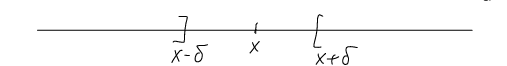
\includegraphics[0.5]{intervalleBoule.png}
       \end{center}
       

   \end{subparag} 
\end{parag}

\begin{parag}{Intérieur d'une boule}
    \begin{definition}
        Soit $E \subset \mathbb{R}^n $ non vide. Alors $ \overline{x} \in E$ est un \important{point intérieur} de $E$ s'il existe $ \delta > 0$ tel que $B( \overline{x}, \delta) \subset E$. L'ensemble des points intérieurs est appelé \important{intérieure} de $E$. Notation $ \mathring{E}$
    \end{definition}
   \begin{subparag}{Remarque personnelle}
       \begin{framedremark}
           On voit ici clairement que $ \mathring{E} < E$. Cette relation est vrai grâce au $ \delta$ qui rend \textit{"plus petit"} notre point $ \overline{x}$
       \end{framedremark}
   \end{subparag}
   Soit $E \subset \mathbb{R}^n $ non vide. Alors $E subset \mathbb{R}^n $ est ouvert $\iff E = \mathring{E}$
   \begin{subparag}{Exemple 1}
       La boule ouverte $B( \overline{x}, \delta) = \{ \overline{y} \in \mathbb{R}^n : \mid  \mid \overline{x} - \overline{y} \mid \mid < \delta \}$ est un sous-ensemble ouvert.\\
       Soit $ \overline{y} \in B( \overline{x}, \delta)$ Alors $ \delta = \frac{1}{2}( \delta - \mid  \mid x - y \mid \mid)  > 0$ implique que:
       \begin{align*}
         &\implies  B( \overline{y}_1, \delta_1) \subset B( \overline{x}, \delta) \\
         &\implies B( \overline{x}, \delta) \subset \mathbb{R}^n 
       \end{align*}
       est un sous-ensemble ouvert de $ \mathbb{R}^n $ $ \forall \overline{x} \in \mathbb{R}^n $, $ \forall \delta > 0$
   \end{subparag}
   \begin{subparag}{Exemple 2}
       Soit $n \geq 2$, $E = \{ \overline{x} \in \mathbb{R}^n  : x_1 = 0, x_i > 0, i = 2, \dots n\} \subset \mathbb{R}^n $
       Ici, nous voulons monter qu'il n'est pas ouvert. \\
       Prenons le point $ \overline{y} = (0, y_2, \dots, y_n)$ où $y_2, \dots, y_n > 0$. Alors pour tout $ \delta > 0$:
       \begin{align*}
           B( \overline{y}, \delta) \ni ( \frac{ \delta}{2}, y_2, \dots, y_n) \notin E
       \end{align*}
       
       
   \end{subparag}
   \begin{subparag}{Exemple 3}
       $\emptyset$ et $ \mathbb{R}^n  \subset \mathbb{R}^n $ sont des sous-ensembles ouverts.      \\
       Ici on a deux cas de figure, 
       \begin{itemize}
           \item $ emptyset$: alors le sous-ensemble est ouvert par définition
           \item Sinon, soit $ \overline{x} \in \mathbb{R}^n $ alors $B( \overline{x}, \delta) \subset \mathbb{R}^n $ et cela: $ \forall \delta > 0$
       \end{itemize}
   \end{subparag}
   \begin{subparag}{Exemple 4}
       $E = \{ \overline{x} \in \mathbb{R}^n: x_i > 0 \forall i = 1, \dots, n\}$\\
       Soit $ \overline{y} \in E$. Alors, nous pouvons prendre $B( \overline{y}, $min$(y_i)) \subset E$.
   \end{subparag}
\end{parag}

\begin{parag}{Propriétés}
    Ici on remarque deux grandes propriétés:
    \begin{enumerate}
       \item Toute réunion $\bigcup_{i \in I} E_i$ des sous-ensembles ouverts est un sous-ensemble ouvert.
           \begin{align*}
               \overline{x} \in \bigcup_{i \in I} E_i \implies \exists j: \overline{x} \in E_j, \; \; E_j \text{ est ouvert } \implies \exists \delta > 0: B( \overline{x}, \delta) \subset E_j \\
               \implies B( \overline{x}, \delta) \subset \bigcup_{i \in I}E_i
           \end{align*}
           

       \item Toute intersection \important{finie} $ \bigcap_{i=1}^nE_i$ des sous-ensembles ouverts est un sous-ensemble ouvert:
            \begin{align*}
               \overline{x} \in  \bigcap_{i\in I}E_i \implies \forall j \overline{x} \in E_j \text{ ouvert } \implies \exists \delta_j > 0 : B( \overline{x}, \delta_j) \subset E_j \\
               \implies B( \overline{x}, \text{min}_j \delta_j) \subset E_j \forall j \implies B( \overline{x}, \text{min} \delta_j) \subset \bigcap_{i=1}^n E_i = E
           \end{align*}
        
    \end{enumerate}
    \begin{framedremark}
        Une intersection infinie des sous-ensembles ouvert de $ \mathbb{R}^n $
    \end{framedremark}
    
\end{parag}



\begin{parag}{Sous-ensemble fermé}
    \begin{definition}
        Soit $E \subset \mathbb{R}^n$ un sous-ensemble. Alors $E$ est \important{Fermé} dans $ \mathbb{R}^n$ si son complément $CE = \{ \overline{x} \in \mathbb{R}^n : \overline{x} \notin E\} = \mathbb{R}^n - E$ est ouvert
    \end{definition}
    
        \begin{align*}
            CB( \overline{x}, \delta) = E \subset \mathbb{R}^n \text{ est fermé}: E = \{ \overline{y} \in \mathbb{R}^n : \mid  \overline{x} - y \mid \geq \delta \} 
        \end{align*}
            Puisque $C(CB( \overline{x}, \delta)) = B( \overline{x}, \delta)$ est ouvert.
\end{parag}
\begin{parag}{Exemples}
    \begin{align*}
        E = \{ \overline{x}\} \subset \mathbb{R}^n 
    \end{align*}
    Ceci est \important{fermé}, car si on prends le complément:
    \begin{align*}
        CE = \{ \overline{y} \in \mathbb{R}^n : \mid \mid \overline{y} - \overline{x} \mid \mid > 0\} \\
        \forall \overline{y} \in CE\; \; \text{la boule} \overline{B}( \overline{y}, \frac{1}{2} \mid  \mid \overline{y} - \overline{x} \mid \mid \subset CE
    \end{align*}
    
    

\end{parag}

\begin{parag}{Question pendant le cours}
    Soient $A$ et $B$ deux sous-ensembles ouverts non-vides de $ \mathbb{R}^n $ Soit $A \setminus B = \{ \overline{x} \in \mathbb{R}^n : \overline{x} \in A \text{ et } \overline{x} \notin B\} $ non-vide.
    \begin{enumerate}
        $A \setminus B$ peut être ouvert, fermé ou ni ouvert ni fermé
        \item $A \setminus$ est soit ouvert, soit fermé
        \item $A \setminus$ ne peut pas être ouvert
        \item $A \setminus$ ne peut pas être fermé
    \end{enumerate}
    Il n'y a qu'une seul possibilité et pour la trouver il faut des contre exemples.

\end{parag}
\begin{parag}{Exemple}
    \begin{align*}
        A = \{(x, y) \in \mathbb{R}^2 : \tan(x + y) \geq 1\}
    \end{align*}
    Et on se pose la question $A$ ouvert, fermé, ni ouvert, ni fermé?
    \\
    Déjà on va trouver tout les valeurs possiblie pour $x$ et $y$ c'est à dire la définition de $\tan$:
    \begin{align*}
        \implies \tan u \text{ existe } \implies u \in ] - \frac{ \pi}{2} + \pi k, \frac{\pi}{2} + \pi k[ \; k \in \mathbb{Z} \\
        \tan u \geq 1 \implies u \in [ \frac{\pi}{4} + \pi k, \frac{\pi}{2} + \pi k[ \; \; \forall k \in \mathbb{Z}
    \end{align*}
   On a donc comme dit auparavant:
   \begin{align*}
       x + y \in  [ \frac{\pi}{4} + \pi k, \frac{\pi}{2} + \pi k[\\
       \frac{\pi}{4} + \pi k \leq x + y < \frac{\pi}{2} + \pi k, k \in \mathbb{Z}\\
       \frac{\pi}{4} + \pi k - x \leq y < \frac{\pi}{2} + \pi k -x
   \end{align*}
   Ici $A$ n'est ni ouvert ni fermé:
   \begin{center}
       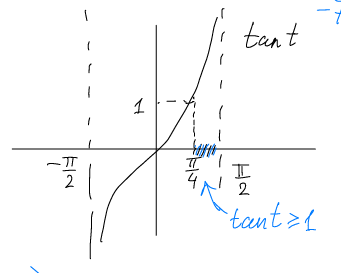
\includegraphics[0.6]{tanBoule.png}
   \end{center}
   \textbf{Explications}: \\
   \begin{enumerate}
       \item $A$ n'est pas ouvert: $(x, y) = (0, \frac{\pi}{4}) = p \in A$
       \begin{align*}
           \forall \delta > 0 \; \; B( \overline{p}, \delta) \text{ contient } (0, \frac{\pi}{4} - \frac{ \delta}{2}) \notin A
       \end{align*}
   \item $A$ n'est pas fermé: $(x, y) = (0, \frac{\pi}{2}) = q \in CA$ 
       \begin{align*}
           \forall \delta > 0 B( \overline{q}, \delta) \text{ contient } (0, \frac{\pi}{2}- \frac{ \delta}{2}) \in A \implies (0, \frac{\pi}{2} - \frac{ \delta}{2}) \notin CA
       \end{align*}
       Et comme $CA$ n'est pas ouvert, alors $A$ n'est pas fermé.
   \end{enumerate}
\end{parag}

\subsection{Méthodes de démonstration: Démonstration par le principe des tiroirs}
\begin{parag}{Principes des tiroirs}
    Si $(n+1)$ objets sont placés dans $n$ tiroirs, alors au moins un tiroir contient $2$ objets ou plus.
    \\
    Plus généralement:
    \begin{theoreme}
        Si $n$ objets sont placés dans $k$ tiroirs, alors au moins un tiroir contient $\left\ceiling \frac{n}{k} \right\ceiling = $min$\{m \in \mathbb{N}: m \geq \frac{n}{k}\}$ objets, ou plus.
    \end{theoreme}
    
    \begin{framedremark}
        Ceci est exactement la même méthode que celle vu en AICC I qu'on appelait le pigeon hole principle, Les preuves sont exactement les mêmes est le but est exactement le même.
    \end{framedremark}
    
\end{parag}


\lecture{8}{2025-02-12}{Suite d'élément de $\mathbb{R}^n$}{}

\begin{parag}{Rappel: Sous-ensembles ouvert et fermmés dans $ \mathbb{R}^n $}
    \begin{definition}
      Soit $E$ un ensemble tel que $E \subset \mathbb{R}^n $ Alors:
      \begin{align*}
          E \subset \mathbb{R}^n  \iff \begin{cases}
              E = \emptyset \\
              E \neq \emptyset \text{et pour chaque point} \overline{x} \in E \text{Il existe} \delta > 0 \text{ tel que } B( \overline{x}, \delta) \subset E
          \end{cases}
      \end{align*}
      
    \end{definition}
    \begin{definition}
        $E \subset \mathbb{R}^n $ est fermé $ \iff$ son complémentaire $CE = \{ \overline{x} \in \mathbb{R}^n : \overline{x} \notin E\}$ est ouvert
    \end{definition}
\end{parag}

\subsection{L'adhérence et la frontière d'un sous-ensemble $ \mathbb{R}^n $}
\begin{parag}{Adhérence}
    \begin{definition}
        Soit $E \subset \mathbb{R}^n $ sous-enesemble non vide. Alors l'intersection de tous les sous-ensembles fermés contenant $E$ est appelée \important{l'adhérence de $E$}.
    \end{definition}
    \begin{subparag}{Notation}
        $ \overline{E}$ est \important{l'adhérence} de $E$ dans $ \mathbb{R}^n $.
        \begin{framedremark}
            Si notre sous-ensemble est déjà fermé alors l'adhérence est égal à lui même:
            \begin{align*}
                E \subset \mathbb{R}^n  \text{fermé} \iff E = \overline{E}
            \end{align*}
            
        \end{framedremark}
        
    \end{subparag}
\begin{definition}
    $E \subset \mathbb{R}^n $ non-vide. $E \neq \mathbb{R}^n $. Un point $ \overline{x} \in \mathbb{R}^n $ est un point de \important{frontière} de $E$ si toute la boule ouverte de centre $x$ cotient au moins un point de  $E$ et au moins un point de $CE$
\end{definition}
L'ensemble des points frontières de $E$ est \important{la frontière de $E$} Notation: $ \partial E$ le d des dérivé partielle.


\end{parag}
\begin{parag}{Exemple}
    \begin{align*}
        E = \{ \overline{x} \in \mathbb{R}^n  : x_i > 0, i = 1, \dots, n\} \implies \partial E = \{ \overline{x} \in \mathbb{R}^n  :  \exists i: x_i = 0, x_j \geq 0 i \neq j\} \\
        \overline{E} = \{ \overline{x} \in \mathbb{R}^n : x_i \geq 0, i = 1, \dots, n\}
    \end{align*}
Soit $E \subset \mathbb{R}^n $ non vide. Alors:
\begin{itemize}
    \item $ \partial E \cap \mathring{E} = \emptyset$
    \item $\mathring{E} \cup \partial E = \overline{E}$ \\
        Ici, on le sait parce que en premier lieu $ \mathring{E} \cup \partial E$ est fermé, et aussi $ E \subset \mathring{E} \cup \partial E$)
    \item $ \partial E = \overline{E} \setminus \mathring{E} = \overline{E} \cup C\mathring{E} \implies \partial E$ est fermé
    \item $ \partial \emptyset = \emptyset$, $ \partial \mathbb{R}^n  = \emptyset$
\end{itemize}
Pourquoi faut il distinguer entre les sous-ensembles ouverts et fermés dans $ \mathbb{R}^n $? La topologie de $ \mathbb{R}^n $ est liée au propriétés des limites des suites d'éléments de $ \mathbb{R}^n $. Et comme la base de l'analyse se base sur la limite, il y a de quoi creuser.

\end{parag}

\subsection{Suites d'éléments de $ \mathbb{R}^n $ et la topologie de $ \mathbb{R}^n $}
\begin{definition}
    \important{Une suite} d'éléments de $ \mathbb{R}^n $ est une application $ f: \mathbb{N} \to \mathbb{R}^n $ 
    \begin{align*}
        f: k \to \overline{x_k} = (x_{1_k}, x_{2_k}, \dots, x_{n_k}) \in \mathbb{R}^n 
    \end{align*}
    Où:
    \begin{align*}
        \{ \overline{x}_k\}_{k=0}^\infty
    \end{align*}
    est une suite d'éléments de $ \mathbb{R}^n $
\end{definition}
\begin{definition}
    $\{ \overline{x}_k\}_{k=0}^\infty$ est \important{convergent} et admet pour \important{limite} $ \overline{x} \in \mathbb{R}^n $ si, pour tout $ \epsilon > 0 \exists k_o \in \mathbb{N}: \forall k \geq k_0, \mid \mid \overline{ \overline{x_k} - \overline{x}} \mid \mid \leq \epsilon$
    Ou alors:
    \begin{align*}
        \overline{x_n} \in \overline{B( \overline{x}, \epsilon} \; \; \forall k \geq k_0
    \end{align*}
    
\end{definition}

\begin{parag}{Remarque}
    soit $ \overline{x} = (x_1, \dots, x_n), \overline{x_k} = (x_{1_k}, \dots, x_{n_k}$, $ \lim_{n \to \infty} \overline{x_k} = \overline{x}$ si et seulement si la limite  $ \lim_{k \to \infty}x_{j_k} = x_j \; \; \forall j= 1, \dots, n$ 

\end{parag}
\begin{parag}{Propriétés}
    \begin{enumerate}
        \item La limite d'une suite $\{ \overline{x}_k\}$, si elle exitste, est unique.
        \item Toute suite convergente $\{ \overline{x_k}\}$ est bornée
            $( \iff $ est contenue dans une boule fermé $ \overline{B( \overline{o}, M)}$
            \begin{align*}
                \lim \overline{x_k} = \overline{x} \implies \exists k_0 \in \mathbb{N}: \forall k \geq k_0 \implies \mid \mid \overline{x} - \overline{x_k} \mid \mid \leq \epsilon \\
                \implies \{ \overline{x_0}, \dots \} \subset \overline{B( \overline{x}, \epsilon)}\\
            \{ \overline{x_0}, \overline{x_1}, \dots, \overline{x}_{k_0-1}\} \cup \{ \overline{x_k}, k \geq k_0\} = \{ \overline{x_k}\}_{k \in \mathbb{N}}
            \end{align*}
            Si nous prenons $M = $ max$\{ \mid \mid \overline{x_i} \mid \mid, i = 0, \dots, k_{o-1}, \mid \mid \overline{x} \mid \mid   + \epsilon\}$
    \end{enumerate}
    

\end{parag}

\begin{parag}{Bolzano-Weierstrass}
    \begin{theoreme}
        De toute suite bornée $\{ \overline{x}_k\} \subset \mathbb{R}^n $ on peut extraire une sous-suite convergente.
    \end{theoreme}
    

\end{parag}
\begin{parag}{Théorème à savoir, Un sous-ensemble non-vide $E \subset \mathbb{R}^n $ est fermé}
\begin{theoreme}
    Un sous-ensemble non vide $E \subset \mathbb{R}^n $ est fermé \important{si et seulement si} toute suite $\{ \overline{x}_k\} < E$ d'élément $E$ qui converge, a pour limite un élément de $E$.
\end{theoreme}
\begin{subparag}{Demonstration $ \implies$ par absurde}
    On cherche dont avec $P$ et $ \neg Q \implies$ absurde
    Soit $ \overline{x} = \lim_{k \to\infty} \overline{x_k}, \overline{x_k} \in E \forall k \in \mathbb{N} $. Supposons par l'absurde que $ \overline{x} \notin E$, $E$ est fermé \\
    ce qui implique que $ \overline{x} \in CE$ où $CE$ est ouvert dans $ \mathbb{R}^n $. Par la définition:
    \begin{align*}
        \exists \delta > 0: B( \overline{x}, \delta) \subset CE \implies \{ \overline{x_k} \forall k \in \mathbb{N}\} \cap B( \overline{x}, \delta) = \emptyset
    \end{align*}
    
    D'autre côté, $ \lim_{k \to \infty} = \overline{x} \implies \exists k_0 \in \mathbb{N}: \forall k \geq k_0, \overline{x}_k \in \overline{B( \overline{x}, \frac{ \epsilon}{2})} \subset B( \overline{x}, \delta)$
\end{subparag}
\begin{subparag}{Contraposé, par contraposé}
    Supposons que $E$ n'est pas fermé, $ \iff$ $CE$ n'est pas ouvert\\
    Alors:
    \begin{align*}
        \implies \exists \overline{y} \in CE \; \forall k \in \mathbb{N}_+ \; \;B( \overline{y}, \frac{1}{k}) \cap E \neq \emptyset\\
        \implies \exists \overline{y_k} \in B( \overline{y}, \frac{1}{k}) \text{ tel que } \overline{y_k} \in E \\
        \text{On a obtenu une suite } \{ \overline{y_k}\}_{k \in \mathbb{N}_+} \subset E \text{ et } \lim_{k \to \infty} \overline{y}_k = \overline{y} \in CE \\
        \iff \overline{y} \notin E\\
        \implies \neq Q \text{ Alors } Q \implies P
    \end{align*}
    

\end{subparag}
\begin{framedremark}
    Pour construire l'adhérence $E$ d'un sous-ensemble non-vide $E \subset \mathbb{R}^n $, il faut et suffit d'ajouter les limites de toues suites convergentes d'éléments de $E$.
\end{framedremark}
    \begin{definition}
        Un sous-ensemble non-vide de $ \mathbb{R}^n $ est \important{compact} s'il est fermé et borné
    \end{definition}
\begin{subparag}{Exemple}
    Soit une boule fermé $ \overline{B( \overline{x}, \delta)} = \{ \overline{y} \in \mathbb{R}^n : \mid \mid \overline{x} - \overline{y} \mid \mid = \delta\}$ Alors $ \overline{B( \overline{x}, \delta)} \subset \overline{B( \overline{o}, \mid \mid \overline{x} \mid \mid+ \delta)}$ est borné. Et donc le sous-ensemble est compact
\end{subparag}
\begin{subparag}{Exemple 2}
    \begin{align*}
        E = \{ \overline{x} \in \mathbb{R}^n : n \geq 2, x_1 = 0\}
    \end{align*}
    est fermé, mais non bornée
    \begin{align*}
        \{ \overline{a}_k = (0, k, 0, \dots)\}_{k \in \mathbb{N}}
    \end{align*}
    Ici les normes $ \mid \mid a_k \mid \mid = k \in \mathbb{N}$. Et donc $CE$ n'est ni borné ni fermé
    
\end{subparag}
\end{parag}
\begin{parag}{Théorème Heine-Borel-Lebesgue}
    \begin{theoreme}
        Un sous-ensemble non-vide $E \subset \mathbb{R}^n $ est compact $ \iff$ de tout recouvrement de $E$ par des sous-ensembles dans $ \mathbb{R}^n $:
        \begin{align*}
            ( E \subset \bigcup_{i \in I} A_i, \; A_i \subset \mathbb{R}^n  \text{ouverts, } A_i \in I \text{ un recouvrement de } E )
        \end{align*}
        On peut extraire une \important{famille finie} d'ensemble que forment un recouvrement de $E$:
        \begin{align*}
            E \subset \bigcup_{i \in I} A_i \; \; A_i \subset \mathbb{R}^n  \text{ ouverts } \implies \exists \{ A_{i_j}\}_{j=1}^m: E \subset \bigcup_{j = 1}^m A_{i_j}
        \end{align*}
    \end{theoreme}
   Ici on peut prendre un nombre infini d'ensemble qui peut recouvrire un nombre fini d'ensemble. Cela ne marche pas si $E$ n'est pas compact.
\begin{subparag}{Exemple 1}
    Une droite dans $ \mathbb{R}^n $, $ n \geq 2$ est fermée, pas bornée $ \implies$ qu'elle n'est pas compacte.
\end{subparag}
\begin{subparag}{Exemple 2}
    Intervalle ouvert dans $  \mathbb{R}$ tel que $E = ] 0, 1 [ \subset \mathbb{R}$ n'est pas fermé ce qui implique que notre ensemble $E$ n'est pas compact
    \begin{align*}
        E \subset \bigcup_{i \in \mathbb{N}} ]0, \frac{i}{i + 1}[
    \end{align*}
    On ne peut pas choisir un sous recouvrement fini. Car si on prends un nombre fini $k$ on dois pouvoir s'arrêter à un $k$ néanmoins ici on n'y arrive pas car on a toujours le nombre $k + 1$
    \begin{framedremark}
        La propriétés d'être compactes est une propriétés très fortes
    \end{framedremark}
\end{subparag}
\end{parag}

\begin{parag}{Exemple}
\begin{subparag}{Exercice}
    \begin{align*}
        A = \{ (x, y) \in \mathbb{R}^2 : \ln (\sin(y-x)) \leq 0\}
    \end{align*}
    Il faut démontrer que $A$ est ouvert.
\end{subparag}
\begin{subparag}{Question 6}
        \begin{align*}
            S = \{ (x, y) \in \mathbb{R}^2: \sqrt{ y \cdot \ln x} < 1\}
        \end{align*}
        \begin{enumerate}
            \item Compact
            \item Ouvert et borné
            \item ni ouvert, ni fermé et non borné
            \item fermé et non borné
            \item ouvert et non borné
            \item ni ouvert, ni fermé et borné
        \end{enumerate}
            
       Pour répondre à cette question, on va prendre tout les cas possibles:
       \begin{enumerate}
           \item $ln x \implies x > 0$
           \item Soit $y = 0 \implies \{ y = 0, x > 0\} \in S$\\
               Aussi $\{ x = 1, y \in \mathbb{R}\} \in S$
           \item Soit $y > 0 \implies y \ln x \geq 0 \implies \ln x geq 0 \wedge x \geq 1$\\
               \begin{align*}
                   y \ln x < 1 \implies y < \frac{1}{\ln x}\\
                   \{y > 0, x > 1, y < \frac{1}{\ln x}\} \subset S
               \end{align*}
           \item Soit $y < 0 \implies y \ln x \geq 0 \implies \ln x \leq 0$ Alors:
               \begin{align*}
                   y \ln x < 1 \implies < \frac{1}{\ln x} \\
                   \{ y < 0, 0 < xx < 1, y > \frac{1}{\ln x}
               \end{align*}
               Ce qui donne comme ensemble:
               \begin{center}
                   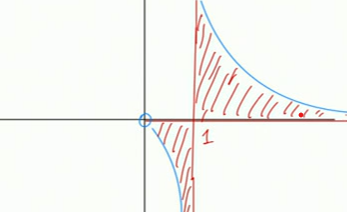
\includegraphics[scale=1.3]{12025-03-12.png}
               \end{center}
               Qui est une droite vertical avec $x = 1$ entre nos deux droite bleu. Néanmoins les lignes bleu ne sont pas inclus, et comme vu sur l'image l'ensemble tends vers les infinis en $x = 1$ et donc, il n'est ni fermé ni borné. Et la raison pour laquelle ce n'est pas ouvert, la  ligne rouge horizontale et fermé et donc ce n'est pas ouvert.
               \begin{framedremark}
                   Attention à faire attention car ici les courbes bleu impliquent que l'ensemble n'est pas fermé mais même si elles étaient fermés, il manquerait quand même le point $0$ qui impliquerait que l'ensemble ne serait pas fermé.
               \end{framedremark}
       \end{enumerate}
\end{subparag}
\end{parag}

\chapter{Fonction réelles de plusieurs variables réelles limite et continuité}
\subsection{Définition et exemples}
\begin{definition}
    Soit $E \subset \mathbb{R}^n $ sous-ensemble non-vide, $n \geq 1$ Une fonction $f : E \to \mathbb{R}$ est une application qui envoie chaque point $ \overline{x} = (x_1, \dots, x_n) \in E$ dans $ \mathbb{R}$. \\
    $E$ est le domaine de définition de $f$ et $f(E)\subset \mathbb{R}$ est l'ensemble image.
\end{definition}
\begin{parag}{Exemple 1}
    \begin{align*}
        f(x, y) = \sqrt{1 - (x^2 - y^2)}
    \end{align*}
    
    
\end{parag}
\begin{parag}{Exemple 2}
    \begin{align*}
        f(x, y) = 2x + 1
    \end{align*}
    Plus généralement:
    \begin{align*}
        f(x, y) = ax + by + c; \; a, b, c, \in \mathbb{R}, E = \mathbb{R}^2
    \end{align*}
  Comment visualiser cette fonction?\\
  \begin{align*}
      \text{Soit } c = 0
  \end{align*}
  Considérons $f(x, y) = ax + by$: Graphique $F = \{(x, y, z): ax + by = z\} = \{(x, y, z) \in \mathbb{R}^3: ax + by -z = 0\} = \{ (x, y, z) \in \mathbb{R}^3: <(x, y, z), (a, b, -1)> = 0\}$ On a donc un plan dont les valeur $a$, $b$ $-1$ sont les composantes d'un vecteur orthogonal: $ \overline{n} = (a, b, -1)$ et contenant $(0, 0, 0)$.
  \\
  Soit $c \in \mathbb{R}$ arbitraire, alors il faut monter le plan par $c$ unité le long de l'axe $z$ pour obtenir le graphique de $f(x, y) = ax+ by + c$ Et donc:
  \begin{align*}
      z = ax + by + x
  \end{align*}
  qui est le plan $ \perp \overline{n} = (a, b, -1)$ qui contient $(0, 0, c)$
  
  
    
\end{parag}
\begin{parag}{Niveau}
    \begin{definition}
        Soit $f : E \to \mathbb{R}$ et $c \in f(E)$ Alors $ \mathcal{N}_f(c) = \{ \overline{x} \in E: f( \overline{x}) = c\} \subset E$
    \end{definition}
    \begin{subparag}{Exemple 4}
        \begin{align*}
            f(x, y) &= \sin(x^2 + y) : E = \mathbb{R}^2\\
            f(E) &= [-1, 1]
        \end{align*}
        
        \begin{framedremark}
            Je conseil de taper sur google les fonctions pour avoir une bonne visualisation de ces fonctions:
            \begin{center}
                \href{https://www.google.com/search?q=sin(x%5E2+%2B+y)&oq=sin(x%5E2+%2B+y)&gs_lcrp=EgZjaHJvbWUyBggAEEUYOTIICAEQABgWGB4yCAgCEAAYFhgeMggIAxAAGBYYHjIICAQQABgWGB4yCAgFEAAYFhgeMgYIBhBFGDwyBggHEEUYPNIBCDM0MDlqMGo0qAIAsAIB&sourceid=chrome&ie=UTF-8}{google.com}
            \end{center}
            
        \end{framedremark}
        On cherche donc les niveaus:
        \begin{align*}
            \mathcal{N}_f(1) &= \{x, y) \in \mathbb{R}^2: \sin(x^2 + y) = 1\}  \\
                             &= \{(x, y) \in \mathbb{R}^2: x^2 + y = \frac{\pi}{2} + 2k\pi, k \in \mathbb{Z}\}\\
                             &= \{(x, y) \in \mathbb{R}^2: y = -x^2 + \frac{\pi}{2} + 2k\pi, k \in \mathbb{Z}
        \end{align*}
        
        
    \end{subparag}

\end{parag}





















\lecture{9}{2025-03-15}{Limite est continuité}{}
\begin{parag}{Rappel}
    \begin{definition}
        Soit $E \subset \mathbb{R}^n $ sous-ensemble non vide, $n \geq 1$ Une fonction est une application qui envoie chaque point $ \overline{x0} = (x_1, \dots, x_n) \in E$ dans $ \mathbb{R}$.\\
        $E$ est le domaine de définition de $f$ et $f(E) \subset \mathbb{R}$ est l'ensemble image.
    \end{definition}
    

\end{parag}

\subsection{Limites et continuité}
\begin{definition}
    Une fonction \important{définie au voisinage de $\overline{x_0}$} (mais pas nécéssairement en $ \overline{x_0}$ tel que
    \begin{align*}
        [ \exists \delta > 0: B( \overline{x}_0, \delta) \subset E \cup \{ \overline{x_0}\}]
    \end{align*}
    admet pour \important{limite} le nombre réel $l$ lorsque $ \overline{x}$ tend vers $ \overline{x_0}$ si \important{pour tout $ \epsilon > 0 \exists \delta > 0$ tel que pour tout $ \overline{x}\in E$ et $0 < \mid \mid \overline{x} - \overline{x}_0 \mid \mid \leq \delta$,  on a $ \mid f( \overline{x}) - l \mid \leq \epsilon$} 
\end{definition}


 \begin{parag}{Notation}
     Pour notre notation on utilise comme à notre habitude:
     \begin{align*}
         \lim_{ \overline{x} \to \overline{x_0}}f( \overline{x}) = l
     \end{align*}
     \begin{framedremark}
         Ici on a la norme $  \mid \mid \overline{x} - \overline{x_0} \mid \mid$ à la place de la valeur absolue lorsqu'on parlait de fonction à une variable. 
     \end{framedremark}
     
 \end{parag}
 \begin{parag}{Continuité}
 
 
 \begin{definition}
     Soit $ \overline{x_0} \in E$ un point intérieur de $E$. Alors $f: E \to \mathbb{R}$ est continue en $ \overline{x} = \overline{x_0}$ \important{si et seulement si}
     \begin{align*}
     \lim_{ \overline{x} \to \overline{x_0}} f( \overline{x}) = f( \overline{x_0})
     \end{align*}
     
 \end{definition}
 

 \begin{subparag}{Exemple 1}
     \begin{align*}
         f(x, y) = 2x + y
     \end{align*}
     soit $(x_0, y0) \in \mathbb{R}^2$: Alors 
     \begin{align*}
         \lim_{(x, y) \to (x_0, y_0)} (x + 2y) = x_0 + 2y_0
     \end{align*}
     Soit $ \epsilon > 0$ alors on cherche $ \mid f(x, y) - f(x_0, y_) \mid = \mid  (x + 2y) - (x_0 + 2y_0) \mid$ si on utilise plus la norme ici et la valeur absolue car on est sur le côté à droite. On utilise l'inéégalité triangulaire:
     \begin{align*}
        &\leq \mid x - x_0 \mid + 2 \mid y - y_0 \mid
     \end{align*}
     Ici on peut toujours prendre comme on a que $ \overline{x} - \overline{x_0}$ plus petit que $ \delta$ on doit les gérer ensembles et non séparément. Des lors:
     Dès lors on choisit $ \delta = \frac{ \epsilon}{3}$
        \begin{align*}
        \leq \sqrt{ (x-x_0)^2 + (y-y_0)^2} + 2\sqrt{(x-x_0)^2 + (y-y_0)^2} = 3\sqrt{(x -x_0)^2 + (y-y_0)^2} \leq 3 \delta = 3 \cdot \frac{ \epsilon}{3} = \epsilon
           \end{align*}

 \end{subparag}
 \begin{subparag}{Exemple 2}
     \begin{align*}
         f(x, y) = x \cdot y \\
         f: \mathbb{R}^2 \to \mathbb{R}
     \end{align*}
     Soit $(x_0, y_0) \in \mathbb{R}^2$ Alors $ \lim_{(x, y) \to (x_0, y_0)} x \cdot y = x_0 \cdot y_0$
     
     \textbf{Démonstration:}\\
    Le cas où $x_0 = 0$ est vu en exercice, dès lors, nous traiterons ici le cas où nous supposerons que $x_0 \neq 0$. Soit $ \epsilon > 0$ alors:
    \begin{align*}
        \mid f(x, y) - f(x_0, y_0)\mid &= \mid xy - x_0y_0 \mid  \\
        &= \mid  (x - x_0)y + x_0(y-y_0) \mid\\
        &\leq \mid x-x_0 \mid \cdot \mid y \mid + \mid y-y_0 \mid \cdot \mid x_0 \mid\\
        \mid y - y_0 \mid \cdot \mid x_0\mid \leq \sqrt{ (x-x_0)^2 + (y-y_0)^2} \mid x_0 \mid \leq  \frac{ \epsilon}{2} \implies \delta \leq \frac{ \epsilon}{2 \mid x_0 \mid} (x_0 \neq 0)\\
        \mid x - x_0 \mid y \mid\mid \leq \sqrt{ (x-x_0)^2 + (y-y_0)^2}\cdot \mid y \mid \leq  \delta  ( \mid y_0 \mid + \delta) \leq \frac{ \epsilon}{2}\\
        \leq \frac{ \epsilon}{2}\\
        \implies \delta \leq \frac{ \epsilon}{2( \mid y_0 \mid + 1)}
    \end{align*}
    On peut choisir comme valeur pour $ \delta$:
    \begin{align*}
        \implies \delta = \text{min} \left( \frac{e}{2 \mid x_0 \mid}, \frac{ \epsilon}{2( \mid y_0\mid + 1)} , 1 \right)  \implies \mid f(x, y)  f(x_0, y_0) \mid \leq \frac{ \epsilon}{2} + \frac{ \epsilon}{2} = \epsilon
    \end{align*}
    
    
     
 \end{subparag}
 \end{parag}

 \begin{parag}{Caractérisation de la limite à partir des suites convergentes}
     \begin{theoreme}
         Une fonction $f: E \to \mathbb{R}$ définie au voisinage de $ \overline{x_0}$ admet pour limite $l \in \mathbb{R}$ lorsque $ \overline{x} \to \overline{x_0}$  \important{Si et seulement si} pour toute suite d'élément $\{ \overline{a_k}\}$ de $\{ \overline{x} \in E: \overline{x} \neq \overline{x_0}\}$, qui converge vers $ \overline{x_0}$, la suite $\{f( \overline{a}_k)\}$ converge vers $l$.
         \begin{align*}
             \lim_{ \overline{x} \to \overline{x_0}} f( \overline{x}) = l \iff \lim_{ k \to \infty} f( \overline{a_k}) = l \text{ pour toute suite } \{ \overline{a_k}\} \subset E \setminus \{ \overline{x_0}\}: \lim_{k \to \infty} \overline{a_k} = \overline{x_0}
         \end{align*}
     \end{theoreme}
 \end{parag}
 
 \begin{parag}{Démonstration}
     \begin{subparag}{ $ \implies$ $P \implies Q$}
         Comme ce théorème est une équivalence, nous allons devoir prouver les deux sens. Commençons par $P \implies Q$. Prenons la définition de la limite à gauche:
         \begin{align*}
             &\lim_{ \overline{x} \to \overline{x_0}} f( \overline{x})= l \implies \forall \epsilon > 0 \exists \delta > 0: \forall \overline{x}: 0 < \mid \mid \overline{x} - \overline{x_0} \mid \mid \leq \delta\\
             &\implies \mid f( \overline{x}) - l \mid \leq \epsilon \\
             &\text{Si on a } \{ \overline{a_k}\}: \lim_{k \to \infty} \overline{a_k} = \overline{x_0} \implies \text{  pour } \delta > 0 \exists k_0 : \forall k \geq k_0 \\
             &\implies \mid \mid \overline{a_k} - \overline{x_0} \mid \mid \leq \delta \implies \mid f( \overline{a_k}) - l \mid \leq \epsilon \\
             &\mid  f( \overline{a}_k) - l \mid \leq \epsilon
         \end{align*}
         \begin{framedremark}
             L'idée ici est de prendre le même $ \delta$ sur les deux première lignes.
         \end{framedremark}
         
     \end{subparag}
     \begin{subparag}{$(\impliedby)$ par contraposée}
         Petit rappel pour la contraposée: si on a $ Q \implies P$ alors la contraposé est $ \neg P \implies \neg Q$ donc ici on veut prouver que si la limite n'est pas $l$ alors la limite de $f( \overline{a_k})$ n'est pas non plus $l$.\\
         Supposons donc que $\lim_{ \overline{x} \to \overline{x_0}}f( \overline{x}) \neq l $ Alors:
             \begin{align*}
                 \exists \epsilon > 0: \forall \delta > 0 \exists \overline{x}_\delta: \mid \mid \overline{x_k} - \overline{x_0} \mid \mid \leq \frac{1}{ \delta} \mid \text{ et } \mid f( \overline{x}_\delta) - l \mid > \epsilon
             \end{align*}
             Dès lors, on peut choisir $ \delta = \frac{1}{k}$, $k \in \mathbb{N}^*$  ce qui implique:
             \begin{align*}
                 \exists \overline{x}_k \in E : \mid \mid  \overline{x_k} - \overline{x_0} \mid \mid \leq \frac{1}{k} \text{ et } \mid f( \overline{x_k}) - l \mid > \epsilon
             \end{align*}
             On obtient la suite $\{ \overline{x}_k\}_{k=1}^\infty: \lim_{k \to \infty} \overline{x_k} = \overline{x_0}$ mais $ \mid f( \overline{x_k}) - l \mid > \epsilon \forall k \in \mathbb{N}^*$ Dès lors
             \begin{align*}
                 \implies f( \overline{x}_k) \neq l
             \end{align*}
     \end{subparag}

     \begin{subparag}{Idée générale de la preuve}
         Ici on prends $P$ et \important{Ensuite} $\neg P$ il est important de pouvoir différencier les deux et de pouvoir construite $\neg P$ à partir de $P$.
         
     \end{subparag}
 \end{parag}

 \begin{parag}{Opération algébrique}
     Soit $f, g$ deux fonctions: $ E_{ \mathbb{R}^n } \to \mathbb{R}$ telles que $\lim_{ \overline{x} \to \overline{x_0}}f( \overline{x}) = l_1$ et $\lim_{ \overline{x} \to \overline{x_0}}g( \overline{x}) = l_2$ Alors:
     \begin{enumerate}
         \item $\lim_{ \overline{x} \overline{x_0}} ( \alpha f + \beta g)( \overline{x}) = \alpha l_1 + \beta l_2$
         \item $\lim_{ \overline{x} \to \overline{x_0}} (f \cdot g)( \overline{x}) = l_1 \cdot l_2$ 
         \item Si $l_2 \neq 0$, alors $\lim_{ \overline{x} \to \overline{x_0}}( \frac{f}{g})( \overline{x}) = \frac{l_1}{l_2}$
     \end{enumerate}
    \begin{subparag}{Conclusion}
        Tous les polynômes en plusieurs variables et toutes les fonctions rationnelles sont continues sur leur domaines de définition,
        \begin{framedremark}
            La caractérisation de la limite à partir des suites convergentes est pratique pour montrer qu'une fonction n'admet pas de limite en $ \overline{x_0} \in \mathbb{R}^n $.
        \end{framedremark}
    \end{subparag} 
    \begin{subparag}{Exemple 1}
        \begin{align*}
            f: \mathbb{R}^2 \to \mathbb{R}\\
            f(x, y) = \begin{cases}
                \frac{xy}{x^2 + y^2} \text{ si } (x, y) \neq (0, 0)\\
                0 \text{ si } (x, y) = (0, 0)
            \end{cases}
        \end{align*}
        Soit $ \overline{a_k} = ( \frac{1}{k}, \frac{1}{k}) \to (0, 0)$ qui implique donc pour la limite:
        \begin{align*}
            \lim_{ k \to \infty} f( \overline{a_k}) = \lim_{k \to\infty} \frac{ \frac{1}{k} \cdot \frac{1}{k}}{ \frac{1}{k^2} + \frac{1}{k^2}} = \frac{1}{2}
        \end{align*}
        Dès lors, on peut aussi prendre $ \overline{b_k} = ( \frac{1}{k},0) \to (0, 0)$ qui par le même procédé:
        \begin{align*}
            \lim_{k \to \infty} f( \overline{b_k}) = \lim_{k \to \infty} \frac{ 0 \cdot \frac{1}{k}}{0 + \frac{1}{k^2}} = 0
        \end{align*}
        Et donc, par la caractérisation à partir des suites, $\lim_{(x, y) \to (0, 0)} f(x, y)$ ne peut pas exister.\\
        On peut aussi prendre une autre suite du genre $ \overline{c_k} = ( - \frac{1}{k}, \frac{1}{k}) \implies \lim_{k \to \infty} f( \overline{a_k}) = - \frac{1}{2}$\\
        Alors quelle est la limite $f(x, y)$ en $(0, 0)$
         \begin{center}
     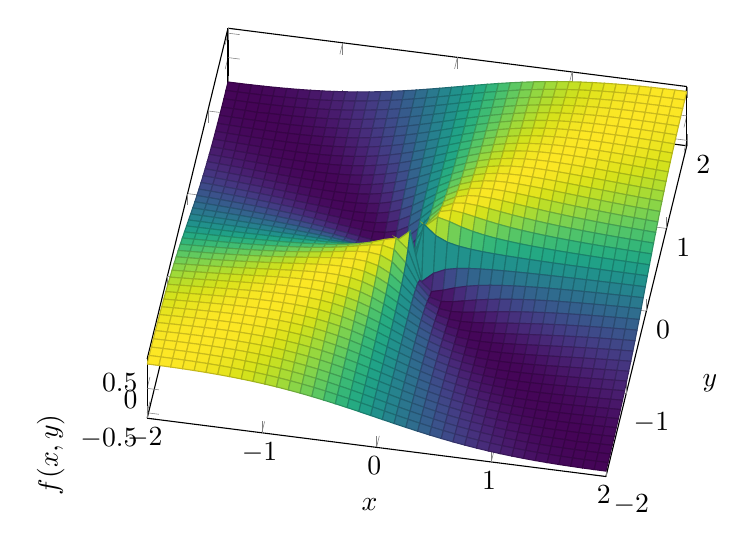
\begin{tikzpicture}
         \begin{axis}[
         view={10}{80},
         domain=-2:2,
         y domain = -2:2,
         colormap/viridis,
         xlabel={$x$},
         ylabel={$y$},
         zlabel={$f(x, y)$},
         samples=40,
         samples y=40,
         ]
         \addplot3[surf] {x*y/(x^2 + y^2)};
     \end{axis}
     \end{tikzpicture}
     
     
 \end{center}
 
    \end{subparag}
    \begin{subparag}{Proposition}
        \begin{theoreme}
            soir $D \subset \mathbb{R}^n $, $f: D \to \mathbb{R}$ définie au voisinage de $ \overline{x_0} \in \mathbb{R}^n $. Alors $\lim_{ \overline{x} \to \overline{x_0}}f( \overline{x}) =l$ si et seulement si pour toute courbe $ y: [a, b] \to \mathbb{R}^n $ telle que:
            \begin{align*}
                 \Upsilon([a, b]) \subset D \setminus\{ \overline{x_0}\} \text{ et } \lim_{t \to a^*} y(t) = \overline{x_0}, \text{ on a } \lim_{t \to a^+} f(y(t)) = l
            \end{align*}
           
        \end{theoreme}
       \begin{framedremark}
           On ne peut pas calculer la limite d'une fonction de plusieurs variable en faisant de manière consecutive par rapport à chaque variable.

       \end{framedremark}
        
    \end{subparag}

    \begin{subparag}{Exemple 2}
        \begin{align*}
            f(x, y) = \begin{cases}
                \frac{x^2 - y^2}{x^2 + y^2} \text{ si } (x, y) \neq (0, 0)\\
                0 \text{ si } (x, y) = (0, 0)
            \end{cases}
        \end{align*}
        Alors on prends deux fonctions;:
        \begin{align*}
            y_1(t) = (t, 0)\\
            y_2(t) = (0, t)
        \end{align*}
        \begin{align*}
            \lim_{t \to o}( \gamma_1(t)) = \lim_{t \to o} \frac{t^2 - 0}{t^2 + 0} = 1\\
            \lim_{t \to 0}f( \gamma_2(t)) = \lim_{t \to 0} \frac{0 - t^2}{0 + t^2} = -1
        \end{align*}
       Et donc la fonction n'a pas de limite en ce point.
    \end{subparag}
    \begin{subparag}{Exemple 3}
        soit:
        \begin{align*}
            f: \mathbb{R}^2 \to \mathbb{R}\\
            f(x, y) = \begin{cases}
                \frac{x^3 + y^3}{x^2 + y^2}\\
                0
            \end{cases}
        \end{align*}
        En prenant les mêmes fonctions:
        \begin{align*}
            \gamma_1(t) = (t, 0) \implies \lim_{t \to 0} \gamma_1(t) = \overline{0}, \lim_{t \to 0} \frac{t^3 + 0}{t^2 + 0} = 0\\
            \gamma_2(t) = (0, t) \implies \lim_{ t \to 0} \gamma_2(t) = \overline{0}, \lim_{t \to 0} \frac{0 - t^3}{0 + t^2} = 0\\
                    \gamma_3 (t, t) \implies\lim_{t \to 0} \gamma_3(t) = \overline{0}, \lim_{t \to 0} \frac{t^3 + t^2}{t^2 + t^1} = 0
        \end{align*}
       On voit ici que ces fonctions ont toute la même limite, et si on prenait n'importe quelle autre  fonction la limite existerait toujours.
       \textbf{Hypothèse} $\lim_{(x, y) \to (0, 0)} f(x, y) = \overline{0}$
    \end{subparag}
 \end{parag}
 
 \begin{parag}{Méthode de changement de variables polaires}
     On peut démontrer l'existence de cette limite par le changement de variables en coordonnées polaires.:
     \begin{align*}
         x = r\cos \phi \text{ si } r \in \mathbb{R}_{ \geq 0}\\
         y = r\sin \phi \text{ si } r \neq 0
     \end{align*}
     Alors on a:
     \begin{align*}
         f(x, y) &= \frac{x^3 + y^3}{x^2 + y^2} \implies f(r, \phi) = \frac{r^3\cos^3\phi + r^3\sin^3\phi}{r^2\cos^2\phi + r^2\sin^2\phi}\\
         &= \frac{r^2(cos^3\phi + \sin^3\phi)}{r^2}\\
         &= r(cos^3\phi + \sin^3\phi)
     \end{align*}
     Ici, $\phi(r)$ est une fonction inconnue, elle pourrait être n'importe quoi.
     \begin{align*}
         \lim_{(x, y) \to (0, 0)}f(x, y) = \lim_{r \to 0} \Phi(r, \phi)\\
         \lim_{r \to 0}\mid r (cos^3\phi + \sin^3\phi) \mid = 0\\
         \implies \lim_{(x, y) \to (0, 0)} f(x, y) = 0
     \end{align*}
     
     
     \begin{framedremark}
         Cette méthode est efficace pour montrer l'existence des limites pour des fonctions de seulement deux variables, et qui tendent vers $(0, 0)$ tel que $\lim_{(x, y) \to (0, 0)} f(x, y)$
     \end{framedremark}
     
     
 
 \end{parag}
\begin{parag}{Théorème des $2$ gendarme}
    \begin{theoreme}
        Soit $f, g, h: E^{\subset \mathbb{R}^n } \to \mathbb{R}$ telles que:
        \begin{enumerate}
            \item $\lim_{ \overline{x} to \overline{x_0}}f( \overline{x}) = \lim_{ \overline{x} \to \overline{x_0}} g( \overline{x}) = l$
            \item Il existe $ \alpha > 0$ pour tout $x \in \{ x \in E: o < \mid \mid \overline{x}- \overline{x_0} \mid \mid \leq \alpha\}$ on a:
                \begin{align*}
                    f( \overline{x}) \leq h( \overline{x}) \leq g( \overline{x})
                \end{align*}
       Alors:
       \begin{align*}
           \lim_{ \overline{x} \to \overline{x_0}}h( \overline{x}) = l
       \end{align*}
        \end{enumerate}
    \end{theoreme}
    
\end{parag}
 
\begin{parag}{Critère des $2$ gendarmes en coordonnées polaires}
    \begin{subparag}{Proposition}
        Soit $D \subset \mathbb{R}^2, f: D \to \mathbb{R}$ définie au voisinage de $(x_0, y0) \in \mathbb{R}^2$. \\
        Alors
        \begin{align*}
            \lim_{(x, y) \to (x_0, y_0)} f(x, y) = l \text{ si et seulement si}
        \end{align*}
      \begin{align*}
          \exists \delta > 0 \text{ et } \phi: ] 0 , \delta [ \to \mathbb{R}:
      \end{align*}
    \begin{itemize}
        \item $ \forall \phi \in [0, 2\pi] \implies \mid f(x_0, r\cos\phi, y_0 + r\sin\phi) - l \mid \leq \phi(r)$
        \item $\lim_{r \to o^+} \phi(r) = 0$
    \end{itemize}    
    \end{subparag}

    \begin{subparag}{Exemple 5}
       soit 
       \begin{align*}
           f(x, y) = \begin{cases}
               \frac{4xy^2}{x^2 + y^2 + 3y^4} \\
               0
           \end{cases}\\
           f(r\cos\phi, r\sin\phi) = \frac{4r^3\cos\phi\sin^2\phi}{r^2 + 3r^4\cos^4\phi} = \frac{4r^3\cos\phi\sin^2\phi}{r^2(1 + 3r^2\sin^4\phi}\\
           \mid f(r\cos\phi, r\sin\phi) - 0 \mid = \frac{4r^3 \mid \cos\phi\sin^2\phi \mid}{r^2 \mid 1 + 3r^2\sin^4\phi \mid}
       \end{align*}
       On sait ici que la partie du nominateur (la partie en haut j'ai un doute) est toujours plus petite ou égale à 1 et la partie du bas plus grande ou égal à $1$. ce qui nous donne:
       \begin{align*}
           \leq \frac{4r^3}{r^2} = 4r = \Phi(r)
       \end{align*}
       Alors 
        \begin{align*}
            \lim_{r \to 0} \Phi(r) = 0
        \end{align*}
        Ce qui par les $2$ gendarmes en coordonnées polaires nous donne:
        \begin{align*}
            \lim_{(x, y) \to (0, 0)} f(x, y) = (0, 0)
        \end{align*}
    \end{subparag}
\end{parag}
\begin{parag}{Question à la fin du cours (Question 7)}
Soit les fonctions \begin{align*}
    f(x, y) = \begin{cases}
        \frac{cos(xy)(x^2 + \sin(y^2))}{\sqrt{x^2 + y^2}}, \; (x, y) \neq (0, 0)\\ 
        0 , \; \text{ Autrement}
    \end{cases} \\
    g(x, y) = \begin{cases}
        \frac{x^2 + y^4}{y^2 + x^4 + x^6}, \; \text{ si } (x, y) \neq (0, 0)\\
        0, \text{ autrement}
    \end{cases}
\end{align*}
La question est quelle fonction est continue en $(0, 0)$?
\begin{subparag}{Solution $f(x, y)$}
    On passe d'abord en coordonnées polaire:
    \begin{align*}
        f(r\cos\phi, r\sin\phi) = \frac{\cos(r^2\sin\phi\cos\phi)(r^2\cos\phi + \sin(r^2\sin^2\phi))}{r}
    \end{align*}
    On prend ensuite la limite:
    \begin{align*}
        \mid f(r\cos\phi, r\sin\phi) - 0 \mid &= \frac{ \mid \cos(r^2\sin\phi\cos\phi) \mid \mid r^2\cos\phi + \sin(r^2\sin^2\phi) \mid}{r}\\
                                              &\leq \frac{ \overbrace{r^2\cos\phi}^{ \geq r^2} + \mid \overbrace{\sin(r^2\sin^2\phi)}^{\leq \mid r^2\sin^2\phi \mid \leq r^2} \mid}{r}\\
                                              &\leq \frac{2r^2}{r} = 2r
    \end{align*}
    Et donc ici on voit que la limite de la fonction va bien vers $0$. ON peut aussi le \textit{"deviner}" en voyant un $r$ tout seul en bas et une $r^2\cos \dots$ en haut. Cela peut donner quelque indice.
\end{subparag}
\begin{subparag}{Solution $g(x, y)$}
    Pour cette fonction on refait le même procédé mais avant on va tester les limites du type $\lim_{t \to 0}g(0, t)$ et aussi $\lim_{t \to 0}g(t, 0)$ et on voit qu'elle ne donne pas la même réponse et que donc, la limite n'existe pas. 
    
\end{subparag}
\end{parag}


 
 
        

\lecture{10}{2025-03-19}{Limites de fonctions}{}
\begin{parag}{Rappel}
    Voici un petit tappel sur les méthodes de calcul des limites de fonction $f: E_{ \subset \mathbb{R}^2} \to \mathbb{R}$
    \begin{enumerate}
        \item s'il existent $2$ suites $ \overline{a_k}$ et $ \overline{b}_k \subset E \setminus\{ \overline{x_0}\}: \lim_{ k \to \infty} \overline{a_k} = \overline{x_0}, \lim_{k \to \infty} \overline{a_k} = \overline{x_0}$ et que, $\lim_{k \to \infty}f( \overline{a_k}) \neq \lim_{k \to \infty} f( \overline{b_k})$ Alors la limite
            \begin{align*}
                \lim_{ \overline{x} \to \overline{x_0}} f( \overline{x})
            \end{align*}
            n'existe pas
        \item S'il existent $2$ courbe $ \gamma_1, \gamma_2: [a, b] \to E \setminus \{ \overline{x_0}\}$ tel que:
            \begin{align*}
                \lim_{t \to a^+} \gamma_1(t) = \lim_{ t \to a^+} \gamma_2(t) = \overline{x_0}
            \end{align*}
            Et que:
            \begin{align*}
               \lim_{t \to a^+}f( \gamma_1(t)) \neq \lim_{t \to a^+} f( \gamma_2(t))
            \end{align*}
            Alors, la limite $ \lim_{ \overline{x} \to \overline{x_0}}f( \overline{x})$ n'existe pas. 
        \item Deux gendarmes: soit $f, g, h: E \to \mathbb{R}$ telles que 
            \begin{align*}
                    \lim_{ \overline{x} \to \overline{x}_0} f( \overline{x}) = \lim_{ \overline{x} \to \overline{x}_0} g( \overline{x})= l
            \end{align*}
            Et que $ \exists \alpha > 0:\; \forall x \in \{x \in E: 0 < \mid \mid \overline{x}- \overline{x_0} \mid \mid < \alpha\}$ on a
            \begin{align*}
                f( \overline{x}) \leq h( \overline{x}) \leq g( \overline{x})
            \end{align*}
            Alors, $h( \overline{x}) = l$
        \item Coordonnées polaires: $f: E \to \mathbb{R}$. Alors $ \lim_{r \to o} f( r\cos\phi, r\sin\phi) = 0 \iff \lim_{(x, y) \to (0, 0)} f(x, y) = 0$ 
            \important{Ici $\phi = \phi(r)$ est une fonction inconnue de $r$}
        \item Deux gendarmes en coordonnées polaires: $f: E \to \mathbb{R}$\\
           \begin{align*}
               \lim_{(x, y) \to (0, 0)} f(x, y) = l \iff \exists \delta > 0 \text{ et } \Phi : ]0, \delta[ \to \mathbb{R}\\
               \forall \phi \in [0, 2\pi], \; \; \forall r \in ]0, \delta [ \text{ on a } \mid f(r\cos\phi, r\sin\phi) - l \mid \leq \Phi(r) \\
               \text{ et } \lim_{r \to o^+} \Phi(r) = 0
           \end{align*}
    \end{enumerate}
    

\end{parag}

\begin{parag}{Développement limité}

    Pour calculer des limites, on peut aussi utiliser les DL connus pour les fonctions d'une seule variables pour trouver des estimations pour les deux gendarme.\\
    Notemment, dans les limites lorsque $ \mid \mid (x, y) - (0, 0) \mid \mid \to 0$ on peut remplacer des expression $\Phi(x)$, $\phi(x)$ par leur DL autour de $x = 0$ ou $y = 0$:
    \begin{align*}
        \Phi(t) = \sum_{k= 0}^n a_\alpha x^k + x^n \cdot \epsilon(x) \text{ 1 seule variable}\\
        x(y) = \sum_{k=0}^n b_k y^k + y^n \cdot \epsilon(y), \dots
    \end{align*}
   On peut composer une fonction d'une seule variable 
   \begin{subparag}{Proposition}
       oit $D \subset \mathbb{R}^2, \: (x_0, y_0) \in D, g:D \to \mathbb{R}$ définie au voisinage de $(x_0, y_0)$, telle que 
       
   \end{subparag}
\end{parag}



\end{document}
